\chapter{Complex Numbers and the Exponential}\label{ch:complex}

\begin{chapterintro}
The numbers at the center of this book are not ordinary real numbers. The $n$-th nontrivial zero of the Riemann zeta function is written $\rho_n=\tfrac12+i t_n$, where $i$ is a number whose square is $-1$. The list $t_1=14.134725$, $t_2=21.022040,\dots$ that you met in Chapter~\ref{ch:intro} is the list of \emph{imaginary parts} of these zeros. The formula that predicts the zeros so well in the paper contains terms like $\sin(mt\log p)/(m\,p^{m/2})$. As you will see in this chapter, each such term is, up to the factor $-1/m$, the imaginary part of a complex power $p^{-ms}$ evaluated at $s=\tfrac12+it$: an arrow that turns around a circle as $t$ increases. To read even the first sentence of the paper you need complex numbers. To understand where its prime-number formula comes from you need the complex exponential.

This chapter builds that language from the ground up. We define $i$ and the arithmetic of complex numbers, draw them as points and arrows in a plane, and describe them by a length and an angle. Then we derive Euler's formula $e^{i\theta}=\cos\theta+i\sin\theta$, the single most useful identity in this book. With it, rotations, oscillations, logarithms and powers like $p^{-s}$ all become simple. We end with functions of a complex variable, their zeros, and the way the angle (``argument'') of a product splits into a sum of angles. That last fact is how the primes enter the counting of zeros later in the book.

Where this shows up in the paper: the notation $\rho_n=\tfrac12+it_n$ in the first sentence of Sec.~I; the sine terms and the factor $p^{-m/2}$ in Eq.~(4); the frequencies $\log p^m$ of Sec.~IV and of the fitted controls in Sec.~II~D; the period $2\pi/\log 2\approx 9$ quoted in Sec.~V; the complex eigenvalues of the non-Hermitian operators $H+iA$ in Secs.~II~E and~V; and the ``phase-randomized'' surrogates of Sec.~III.
\end{chapterintro}

\begin{prerequisites}
\item Chapter~\ref{ch:intro}: the list of zeros $t_1, t_2,\dots$ (running example RE1) and the outline of the paper's question.
\item First-year physics and calculus: trigonometric functions and the addition formulas $\cos(a+b)=\cos a\cos b-\sin a\sin b$ and $\sin(a+b)=\sin a\cos b+\cos a\sin b$; $\cos^2\theta+\sin^2\theta=1$; $\cos$ is even and $\sin$ is odd.
\item Derivatives of $e^x$, $\sin x$, $\cos x$; the natural logarithm $\log x$ as the inverse of $e^x$ (in this book $\log$ always means the natural logarithm).
\item Two-dimensional vectors: components, magnitude, the angle a vector makes with the $x$ axis.
\item Uniform circular motion and simple harmonic motion (SHM) as its projection; angular frequency $\omega$ and period $2\pi/\omega$.
\item The finite geometric sum $1+r+r^2+\dots+r^{n-1}=(r^n-1)/(r-1)$ for $r\neq1$.
\end{prerequisites}

%==========================================================
\section{Why a new kind of number?}\label{sec:complex-why}
% DYK-BEGIN
\begin{didyouknow}{Ten Split Into Two}
In his 1545 book \emph{Ars Magna}, Gerolamo Cardano asked for two numbers that add to 10 and multiply to 40. The answer, $5+\sqrt{-15}$ and $5-\sqrt{-15}$, struck him as subtle but useless. Yet his cubic formula sometimes passed through square roots of negative numbers even when the final roots were real. In 1572 Rafael Bombelli showed how to calculate with them consistently.
\end{didyouknow}
% DYK-END

Try to solve $x^2+1=0$. You need a number whose square is $-1$. No real number works: the square of a positive number is positive, the square of a negative number is positive, and $0^2=0$. So within the real numbers this equation has no solution at all.

Mathematicians did not invent a new number just to be stubborn about such equations. In the sixteenth century, Italian algebraists found that their formulas for solving cubic equations sometimes passed \emph{through} square roots of negative numbers on the way to perfectly ordinary real answers. The square roots of negatives were a useful intermediate tool even when nobody believed in them. Over the following centuries it became clear that the extended number system is consistent, and that it is the natural language for anything that rotates or oscillates.

That last point is why physicists care. An oscillation $\cos\omega t$ is the shadow of a point going around a circle (you met this in first-year physics: SHM is the projection of uniform circular motion). Complex numbers let us work with the whole circle instead of its shadow, and the circle is much easier to compute with. Alternating-current circuits, waves, and all of quantum mechanics (Chapter~\ref{ch:schrodinger}) are written in complex numbers for this reason.

For us there is a further reason. The Riemann zeta function, from which our mysterious list of numbers comes, is a function of a \emph{complex} variable $s$. Its zeros are complex numbers. And the primes enter through quantities $p^{-s}$, which on the vertical line where all the computed zeros sit are arrows of fixed length turning at a rate set by $\log p$. By the end of this chapter you will be able to compute such arrows, add them, and take their angles.

\begin{keyideas}
\item Some equations, like $x^2+1=0$, have no real solutions. We extend the number system by adding a number $i$ with $i^2=-1$.
\item Complex numbers are the natural language of rotation and oscillation.
\item The zeta zeros $\rho_n=\tfrac12+it_n$ are complex numbers, and the primes enter the theory through complex powers $p^{-s}$.
\end{keyideas}

%==========================================================
\section{The imaginary unit and complex arithmetic}\label{sec:complex-arith}

\subsection{Definitions}

We introduce a new number, the \textbf{imaginary unit} $i$, defined by the single property
\begin{equation}
i^2=-1.\label{eq:complex-i}
\end{equation}
A \textbf{complex number} is an expression
\begin{equation}
z=a+bi,\qquad a,b\ \text{real numbers}.\label{eq:complex-z}
\end{equation}
The real number $a$ is called the \textbf{real part} of $z$, written $\Re z=a$. The real number $b$ is called the \textbf{imaginary part} of $z$, written $\Im z=b$. We also write $a+ib$ for $a+bi$; the order of the factors $b$ and $i$ does not matter. A complex number with $b=0$ is just the real number $a$, so every real number is also a complex number. A complex number with $a=0$, such as $3i$, is called \textbf{purely imaginary}.

Two complex numbers are \textbf{equal} when both their real parts are equal and their imaginary parts are equal:
\begin{equation}
a+bi=c+di\quad\Longleftrightarrow\quad a=c\ \text{and}\ b=d.\label{eq:complex-equal}
\end{equation}
So one complex equation is really \emph{two} real equations. Keep this in mind; it will matter when we look for zeros of complex functions.

\begin{pitfall}
The imaginary part of $z=a+bi$ is the \emph{real} number $b$, not $bi$. For example $\Im(3-4i)=-4$. When the paper writes $\rho_n=\tfrac12+it_n$ and calls $t_n$ the ``imaginary part'', $t_n$ is an ordinary real number such as $14.134725$.
\end{pitfall}

\subsection{Addition, subtraction, multiplication}

We add and subtract complex numbers part by part:
\begin{align}
(a+bi)+(c+di)&=(a+c)+(b+d)i,\label{eq:complex-add}\\
(a+bi)-(c+di)&=(a-c)+(b-d)i.\nonumber
\end{align}
To multiply, we use the ordinary distributive law of algebra, treating $i$ as a symbol, and then replace $i^2$ by $-1$ using Eq.~\eqref{eq:complex-i}:
\begin{align}
(a+bi)(c+di)&=ac+a(di)+(bi)c+(bi)(di)\nonumber\\
&=ac+adi+bci+bd\,i^2\nonumber\\
&=ac+adi+bci-bd\quad\text{(using $i^2=-1$)}\nonumber\\
&=(ac-bd)+(ad+bc)i.\label{eq:complex-mult}
\end{align}
Look at the final line: if you swap $(a,b)$ with $(c,d)$, the real part $ac-bd$ and the imaginary part $ad+bc$ do not change. So complex multiplication is commutative, $zw=wz$. The distributive law $z(w+u)=zw+zu$ also holds. With $z=a+bi$, $w=c+di$, $u=e+fi$, Eq.~\eqref{eq:complex-add} gives $w+u=(c+e)+(d+f)i$, so by Eq.~\eqref{eq:complex-mult}
\begin{align*}
z(w+u)&=\bigl[a(c+e)-b(d+f)\bigr]+\bigl[a(d+f)+b(c+e)\bigr]i\\
&=\bigl[(ac-bd)+(ae-bf)\bigr]+\bigl[(ad+bc)+(af+be)\bigr]i ,
\end{align*}
which by Eqs.~\eqref{eq:complex-mult} and \eqref{eq:complex-add} is $zw+zu$. The associative law $(zw)u=z(wu)$ holds too: expanding both sides with Eq.~\eqref{eq:complex-mult} produces the same real products in each part. Problem~9 asks you to carry out this expansion in general and for a concrete case. The upshot is that you may manipulate complex numbers with all the familiar rules of algebra, remembering only that $i^2=-1$.

\subsection{Powers of $i$}

The powers of $i$ repeat with period 4:
\begin{equation}
i^0=1,\quad i^1=i,\quad i^2=-1,\quad i^3=i^2\cdot i=-i,\quad i^4=i^2\cdot i^2=(-1)(-1)=1,\label{eq:complex-ipowers}
\end{equation}
and then $i^5=i^4\cdot i=i$, $i^6=-1$, and so on. To find $i^n$, divide $n$ by 4 and keep the remainder. Also $i^{-1}=1/i$; since $i\cdot(-i)=-i^2=1$, we have $i^{-1}=-i$. This cycle of four will be the engine of Euler's formula in Section~\ref{sec:complex-euler}.

\begin{sample}{Multiplying complex numbers}
Compute $zw$ for $z=3+2i$ and $w=1-4i$, and compute $i^{27}$.

\textbf{Step 1:} Expand the product: $(3+2i)(1-4i)=3\cdot1+3\cdot(-4i)+2i\cdot1+2i\cdot(-4i)=3-12i+2i-8i^2$.

\textbf{Step 2:} Replace $i^2$ by $-1$: $-8i^2=+8$. So the product is $3+8+(-12+2)i=11-10i$.

\textbf{Step 3:} Check with Eq.~\eqref{eq:complex-mult}, $a=3$, $b=2$, $c=1$, $d=-4$: real part $ac-bd=3-(-8)=11$; imaginary part $ad+bc=-12+2=-10$. Agreed.

\textbf{Step 4:} For $i^{27}$: $27=4\cdot6+3$, so $i^{27}=(i^4)^6\,i^3=1\cdot(-i)$.

\[
\boxed{(3+2i)(1-4i)=11-10i,\qquad i^{27}=-i}
\]
\end{sample}

\begin{pitfall}
Do not use the rule $\sqrt{x}\sqrt{y}=\sqrt{xy}$ with negative $x,y$. If we agree that $\sqrt{-1}$ means $i$, then $\sqrt{-1}\sqrt{-1}=i^2=-1$, but $\sqrt{(-1)(-1)}=\sqrt1=1$. The rule is true only for nonnegative real numbers. In this book we avoid writing square roots of negative numbers except in the quadratic formula, where we say exactly which root we mean.
\end{pitfall}

\begin{checkpoint}
Is $i$ a real number? What is $i^2\cdot i^2$?
\end{checkpoint}
\checkanswer{No: no real number squares to $-1$. And $i^2\cdot i^2=(-1)(-1)=1$, which is $i^4$.}

\subsection{Complex numbers in Python}

Python has complex numbers built in. It follows the engineering convention of writing the imaginary unit as \texttt{j}, so $3+2i$ is typed \texttt{3 + 2j}. (Appendix~A explains how to run such snippets.)

\begin{pycode}
z = 3 + 2j            # Python writes i as j
w = 1 - 4j
print(z + w)          # (4-2j)
print(z * w)          # (11-10j)
print(z.real, z.imag) # 3.0 2.0  (both are real numbers)
print(1j**2)          # (-1+0j)
\end{pycode}

\begin{keyideas}
\item The imaginary unit satisfies $i^2=-1$. A complex number is $z=a+bi$ with real part $\Re z=a$ and imaginary part $\Im z=b$, both real.
\item Two complex numbers are equal when both parts agree, so one complex equation is two real equations.
\item Add part by part; multiply by expanding and using $i^2=-1$: $(a+bi)(c+di)=(ac-bd)+(ad+bc)i$, Eq.~\eqref{eq:complex-mult}.
\item Powers of $i$ cycle: $1,i,-1,-i,1,\dots$.
\end{keyideas}

%==========================================================
\section{The complex plane: modulus and conjugate}\label{sec:complex-plane}

\subsection{Points and arrows}

A complex number $z=a+bi$ is fixed by two real numbers $(a,b)$. So we can draw it as the point with coordinates $(a,b)$ in a plane, or as the arrow (two-dimensional vector) from the origin to that point. This picture is called the \textbf{complex plane} (or Argand diagram). The horizontal axis is the \textbf{real axis}; the vertical axis is the \textbf{imaginary axis}. \Cref{fig:complex-plane} shows several examples.

The picture makes addition familiar. By Eq.~\eqref{eq:complex-add}, adding complex numbers adds their components, which is exactly how you add vectors in first-year physics: place the arrows head to tail (the parallelogram rule).

\begin{figure}[htbp]\centering
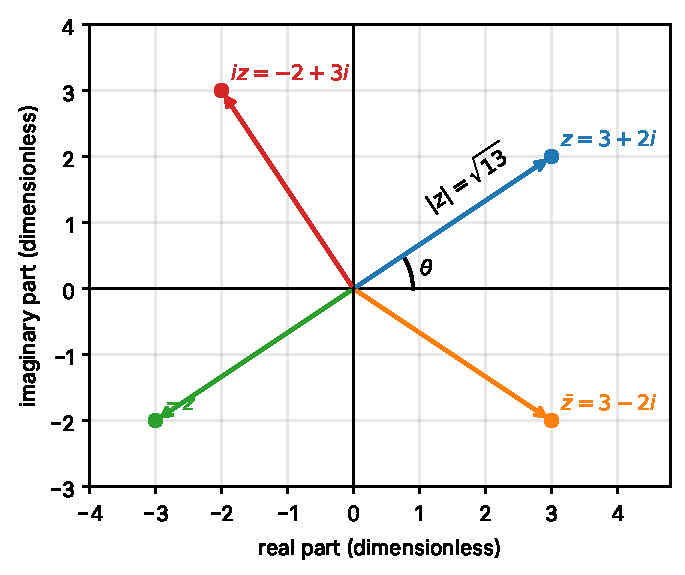
\includegraphics[width=0.85\linewidth]{figs/complex_plane.pdf}
\caption{The complex plane. The number $z=3+2i$ is the point $(3,2)$, or the arrow from the origin to it. Its length is the modulus $\abs{z}=\sqrt{13}$ and its angle from the positive real axis is the argument $\theta=\arg z$. The conjugate $\bar z=3-2i$ is the mirror image in the real axis; $-z$ is the arrow reversed; and $iz=-2+3i$ is $z$ rotated by $90^\circ$ counterclockwise.}
\label{fig:complex-plane}
\end{figure}

\subsection{The complex conjugate}

The \textbf{complex conjugate} of $z=a+bi$ is
\begin{equation}
\bar z=a-bi.\label{eq:complex-conj}
\end{equation}
(Some books write $z^*$; the paper does not need either symbol, but later chapters on quantum mechanics use both.) Geometrically, $\bar z$ is the reflection of $z$ in the real axis. Reflecting twice returns the original point: $\overline{\bar z}=\overline{a-bi}=a+bi=z$. Three identities follow directly by writing out the parts:
\begin{align}
z+\bar z&=(a+bi)+(a-bi)=2a=2\Re z,\label{eq:complex-zpluszbar}\\
z-\bar z&=(a+bi)-(a-bi)=2bi=2i\Im z,\nonumber\\
z\bar z&=(a+bi)(a-bi)=a^2-abi+abi-b^2i^2=a^2+b^2.\label{eq:complex-zzbar}
\end{align}
The last line is important: $z\bar z$ is always a real number, and it is never negative.

Conjugation respects arithmetic. With $z=a+bi$ and $w=c+di$, Eq.~\eqref{eq:complex-mult} gives $zw=(ac-bd)+(ad+bc)i$, so $\overline{zw}=(ac-bd)-(ad+bc)i$. On the other hand
\[
\bar z\,\bar w=(a-bi)(c-di)=ac-adi-bci+bd\,i^2=(ac-bd)-(ad+bc)i.
\]
The two agree, so
\begin{equation}
\overline{zw}=\bar z\,\bar w,\qquad\text{and similarly}\qquad\overline{z+w}=\bar z+\bar w.\label{eq:complex-conjrules}
\end{equation}

\subsection{The modulus}

The \textbf{modulus} (or absolute value) of $z=a+bi$ is the length of its arrow,
\begin{equation}
\abs{z}=\sqrt{a^2+b^2}.\label{eq:complex-modulus}
\end{equation}
By Pythagoras this is the distance from the origin to the point $(a,b)$; it is the magnitude of the vector $(a,b)$ from first-year physics. For a real number ($b=0$) it reduces to the ordinary absolute value $\sqrt{a^2}=\abs a$. Comparing with Eq.~\eqref{eq:complex-zzbar},
\begin{equation}
z\bar z=\abs{z}^2.\label{eq:complex-zzbar2}
\end{equation}
Also $\abs z=0$ only if $a^2+b^2=0$, which for real $a,b$ forces $a=b=0$, i.e. $z=0$. The distance between two complex numbers $z$ and $w$ in the plane is $\abs{z-w}$, the length of the arrow from $w$ to $z$.

\subsection{Division}

To divide by a nonzero complex number $z$, multiply the top and bottom by $\bar z$ (this multiplies by $\bar z/\bar z=1$, so it changes nothing), and use Eq.~\eqref{eq:complex-zzbar2} to make the bottom real:
\begin{equation}
\frac{w}{z}=\frac{w\,\bar z}{z\,\bar z}=\frac{w\,\bar z}{\abs z^2}.\label{eq:complex-div}
\end{equation}
In particular $1/z=\bar z/\abs z^2$. Dividing by the real number $\abs z^2$ just divides both parts.

\begin{sample}{Dividing complex numbers}
Compute $(3+2i)/(1-4i)$ in the form $a+bi$, and check the answer.

\textbf{Step 1:} The denominator is $z=1-4i$, so $\bar z=1+4i$ and $\abs z^2=1^2+4^2=17$.

\textbf{Step 2:} Multiply the numerator by $\bar z$: $(3+2i)(1+4i)=3+12i+2i+8i^2=3-8+14i=-5+14i$.

\textbf{Step 3:} Divide by 17: $\dfrac{-5+14i}{17}=-\dfrac{5}{17}+\dfrac{14}{17}i\approx-0.294118+0.823529\,i$.

\textbf{Step 4:} Check by multiplying back: $\dfrac{(-5+14i)(1-4i)}{17}=\dfrac{-5+20i+14i-56i^2}{17}=\dfrac{51+34i}{17}=3+2i$. Correct.

\[
\boxed{\frac{3+2i}{1-4i}=\frac{-5+14i}{17}\approx-0.294118+0.823529\,i}
\]
\end{sample}

\subsection{The modulus of a product, and the triangle inequality}

Two inequalities and identities about moduli will be used throughout the book.

\textbf{Modulus of a product.} For any complex $z,w$,
\begin{equation}
\abs{zw}=\abs z\,\abs w.\label{eq:complex-absprod}
\end{equation}
Proof: by Eq.~\eqref{eq:complex-zzbar2} and Eq.~\eqref{eq:complex-conjrules},
\[
\abs{zw}^2=(zw)\overline{(zw)}=z\,w\,\bar z\,\bar w=(z\bar z)(w\bar w)=\abs z^2\abs w^2 .
\]
In the first equality we used Eq.~\eqref{eq:complex-zzbar2} for the complex number $zw$: by definition $\abs{zw}$ is the nonnegative square root of $(zw)\overline{(zw)}$. Both sides of Eq.~\eqref{eq:complex-absprod} are nonnegative, so taking square roots gives the result. Dividing, $\abs{w/z}=\abs w/\abs z$ for $z\ne0$.

\textbf{Triangle inequality.} For any complex $z,w$,
\begin{equation}
\abs{z+w}\le\abs z+\abs w.\label{eq:complex-triangle}
\end{equation}
Geometrically: one side of a triangle is no longer than the other two together. Proof in steps:
\begin{align*}
\abs{z+w}^2&=(z+w)(\bar z+\bar w)\quad\text{(Eqs.~\eqref{eq:complex-zzbar2}, \eqref{eq:complex-conjrules})}\\
&=z\bar z+z\bar w+w\bar z+w\bar w\\
&=\abs z^2+\abs w^2+\bigl(z\bar w+\overline{z\bar w}\bigr)\quad\text{(since $\overline{z\bar w}=\bar z\,\overline{\bar w}=\bar z w$ by Eq.~\eqref{eq:complex-conjrules} and $\overline{\bar w}=w$)}\\
&=\abs z^2+\abs w^2+2\Re(z\bar w)\quad\text{(Eq.~\eqref{eq:complex-zpluszbar})}.
\end{align*}
Now for any complex $u=c+di$, $\Re u=c\le\sqrt{c^2+d^2}=\abs u$. With $u=z\bar w$ and $\abs{z\bar w}=\abs z\abs{\bar w}=\abs z\abs w$ (Eq.~\eqref{eq:complex-absprod}, and $\abs{\bar w}=\abs w$ because changing the sign of the imaginary part does not change $c^2+d^2$),
\[
\abs{z+w}^2\le\abs z^2+\abs w^2+2\abs z\abs w=(\abs z+\abs w)^2 .
\]
Taking nonnegative square roots proves Eq.~\eqref{eq:complex-triangle}.

\subsection{Complex numbers cannot be put in order}

Real numbers can be compared: $2<3$. Complex numbers cannot, at least not in any way that cooperates with multiplication. Suppose there were an ordering in which, as for real numbers, the product of two positive numbers is positive and exactly one of $z$, $-z$ is positive for $z\neq0$. If $i$ were positive, then $i\cdot i=-1$ would be positive, and so would $(-1)(-1)=1$; but then both $1$ and $-1$ are positive, a contradiction. If instead $-i$ were positive, then $(-i)(-i)=i^2=-1$ would be positive, the same contradiction. So the phrase ``the larger of two complex numbers'' has no meaning. This matters later: the eigenvalues of the paper's non-Hermitian operators (Sec.~II~E) can be complex, so they have no natural ``increasing order'' of the kind real energy levels have. In any case, order alone would not tell which perturbed state came from which unperturbed one. The paper identifies states by overlap (Sec.~II~E (iii); Chapter~\ref{ch:non-hermitian}).

\begin{checkpoint}
What is the conjugate of a real number? What does conjugation do to the modulus?
\end{checkpoint}
\checkanswer{A real number $a=a+0i$ is its own conjugate, since $a-0i=a$. Conjugation leaves the modulus unchanged: $\abs{a-bi}=\sqrt{a^2+(-b)^2}=\abs{a+bi}$ (a reflection does not change length).}

\begin{keyideas}
\item A complex number $a+bi$ is the point (or arrow) $(a,b)$ in the complex plane; addition is vector addition.
\item The conjugate $\bar z=a-bi$ is the reflection in the real axis; $\overline{zw}=\bar z\bar w$.
\item The modulus $\abs z=\sqrt{a^2+b^2}$ is the length of the arrow; $z\bar z=\abs z^2$; $\abs{zw}=\abs z\abs w$; $\abs{z+w}\le\abs z+\abs w$.
\item Divide by multiplying top and bottom by the conjugate: $w/z=w\bar z/\abs z^2$.
\item Complex numbers have no ordering compatible with multiplication.
\end{keyideas}

%==========================================================
\section{Polar form and the argument}\label{sec:complex-polar}

\subsection{Length and angle}

An arrow in the plane can be described by its components $(a,b)$, or by its length $r$ and the angle $\theta$ it makes with the positive real axis (measured counterclockwise, in radians). From the right triangle in \Cref{fig:complex-plane},
\begin{equation}
a=r\cos\theta,\qquad b=r\sin\theta,\qquad\text{so}\qquad z=r(\cos\theta+i\sin\theta).\label{eq:complex-polar}
\end{equation}
This is the \textbf{polar form}. The length $r=\abs z$ is the modulus. The angle $\theta$ is called the \textbf{argument} of $z$, written $\arg z$. Physicists also call it the \textbf{phase} of $z$.

The argument is not unique. Adding $2\pi$ to $\theta$ turns the arrow by a full circle and brings it back, so $\theta$, $\theta+2\pi$, $\theta-2\pi$, and in general $\theta+2\pi k$ for any integer $k$ all describe the same $z$. When we need a single definite value we use the \textbf{principal argument}, written $\operatorname{Arg} z$, which is the value in the interval $(-\pi,\pi]$. The argument of $z=0$ is not defined, because the zero arrow points nowhere.

\subsection{Computing the argument without quadrant errors}

From Eq.~\eqref{eq:complex-polar}, $\tan\theta=b/a$ when $a\ne0$. But the inverse tangent $\arctan$ only returns angles in $(-\pi/2,\pi/2)$, the right half of the plane, while $-1-i$ and $1+i$ have the same ratio $b/a=1$ and point in opposite directions. The correct rule for the principal argument of $a+bi\neq0$ is
\begin{equation}
\operatorname{Arg}(a+bi)=
\begin{cases}
\arctan(b/a) & a>0,\\
\arctan(b/a)+\pi & a<0,\ b\ge0,\\
\arctan(b/a)-\pi & a<0,\ b<0,\\
\pi/2 & a=0,\ b>0,\\
-\pi/2 & a=0,\ b<0.
\end{cases}\label{eq:complex-atan2}
\end{equation}
Computers provide this as the two-argument function \texttt{atan2(b, a)}; in numpy, \texttt{np.angle(z)} returns $\operatorname{Arg}z$ directly.

\begin{pitfall}
Never compute an argument as $\arctan(b/a)$ alone. For $z=-1-i$ that gives $\arctan 1=\pi/4$, which points into the first quadrant. The correct principal argument (third line of Eq.~\eqref{eq:complex-atan2}) is $\pi/4-\pi=-3\pi/4$. Always ask which quadrant the point lies in.
\end{pitfall}

\begin{sample}{Modulus and argument of the first zeta zero}
The first nontrivial zero of the zeta function is $\rho_1=\tfrac12+it_1$ with $t_1=14.134725$ (running example RE1). Find $\abs{\rho_1}$ and $\operatorname{Arg}\rho_1$ in radians and degrees.

\textbf{Step 1:} Real part $a=0.5$, imaginary part $b=14.134725$.

\textbf{Step 2:} Modulus: $\abs{\rho_1}^2=0.5^2+14.134725^2=0.25+199.790451=200.040451$, so $\abs{\rho_1}=\sqrt{200.040451}\approx14.1436$.

\textbf{Step 3:} Since $a>0$, the first line of Eq.~\eqref{eq:complex-atan2} applies: $\operatorname{Arg}\rho_1=\arctan(14.134725/0.5)=\arctan(28.26945)$. It is easier to use $\arctan(b/a)=\pi/2-\arctan(a/b)$ for $a,b>0$ (the two acute angles of a right triangle add to $\pi/2$): $\arctan(0.5/14.134725)=\arctan(0.0353739)\approx0.0353592$, so $\operatorname{Arg}\rho_1\approx1.5707963-0.0353592=1.53544$.

\textbf{Step 4:} In degrees: $1.53544\times180/\pi\approx87.974^\circ$.

\[
\boxed{\abs{\rho_1}\approx14.1436,\qquad \operatorname{Arg}\rho_1\approx1.53544\ \text{rad}\approx87.974^\circ}
\]
The zero lies very close to the imaginary axis direction, because its imaginary part is much larger than its real part $\tfrac12$. All the zeros used in the paper sit on the vertical line $\Re s=\tfrac12$ (\Cref{fig:complex-critical} in Section~\ref{sec:complex-paper}).
\end{sample}

\subsection{Multiplying in polar form: moduli multiply, arguments add}

Here is the reason polar form is so useful. Take $z_1=r_1(\cos\theta_1+i\sin\theta_1)$ and $z_2=r_2(\cos\theta_2+i\sin\theta_2)$. Multiply, using Eq.~\eqref{eq:complex-mult} with $a=\cos\theta_1$, $b=\sin\theta_1$, $c=\cos\theta_2$, $d=\sin\theta_2$:
\begin{align}
z_1z_2&=r_1r_2\bigl[(\cos\theta_1\cos\theta_2-\sin\theta_1\sin\theta_2)+i(\cos\theta_1\sin\theta_2+\sin\theta_1\cos\theta_2)\bigr]\nonumber\\
&=r_1r_2\bigl[\cos(\theta_1+\theta_2)+i\sin(\theta_1+\theta_2)\bigr]\quad\text{(addition formulas)}.\label{eq:complex-prodpolar}
\end{align}
So the modulus of a product is the product of the moduli (as already found in Eq.~\eqref{eq:complex-absprod}) and \emph{an argument of the product is the sum of the arguments}:
\begin{equation}
\arg(z_1z_2)=\arg z_1+\arg z_2\quad(\text{up to a multiple of }2\pi).\label{eq:complex-argprod}
\end{equation}
We abbreviate ``up to adding an integer multiple of $2\pi$'' as ``mod $2\pi$''. The phrase ``up to a multiple of $2\pi$'' matters: if $\operatorname{Arg}z_1=3$ and $\operatorname{Arg}z_2=1$, the sum $4$ is outside $(-\pi,\pi]$, and the principal argument of the product is $4-2\pi$.

For quotients, since $z_1=(z_1/z_2)z_2$, Eq.~\eqref{eq:complex-argprod} gives $\arg(z_1/z_2)=\arg z_1-\arg z_2$, and $\abs{z_1/z_2}=r_1/r_2$. For the conjugate, $\bar z=r(\cos\theta-i\sin\theta)=r(\cos(-\theta)+i\sin(-\theta))$ (cosine even, sine odd), so $\arg\bar z=-\arg z$.

\subsection{De Moivre's formula}

Applying Eq.~\eqref{eq:complex-prodpolar} repeatedly to equal factors gives, for every positive integer $n$,
\begin{equation}
(\cos\theta+i\sin\theta)^n=\cos n\theta+i\sin n\theta .\label{eq:complex-demoivre}
\end{equation}
Proof by induction. For $n=1$ there is nothing to prove. Suppose it holds for some $n$. Then
\[
(\cos\theta+i\sin\theta)^{n+1}=(\cos n\theta+i\sin n\theta)(\cos\theta+i\sin\theta)=\cos(n\theta+\theta)+i\sin(n\theta+\theta),
\]
using Eq.~\eqref{eq:complex-prodpolar} with $r_1=r_2=1$. That is the formula for $n+1$, so it holds for all $n\ge1$. Hence $z^n=r^n(\cos n\theta+i\sin n\theta)$: raising to the $n$-th power raises the modulus to the $n$-th power and multiplies the argument by $n$.

\begin{sample}{A power the easy way}
Compute $(1+i)^8$.

\textbf{Step 1:} Polar form: $\abs{1+i}=\sqrt{1+1}=\sqrt2$, and since $a=b=1>0$, $\operatorname{Arg}(1+i)=\arctan1=\pi/4$.

\textbf{Step 2:} By De Moivre, $(1+i)^8=(\sqrt2)^8\bigl[\cos(8\cdot\pi/4)+i\sin(8\cdot\pi/4)\bigr]=16(\cos2\pi+i\sin2\pi)=16(1+0i)$.

\textbf{Step 3:} Check another way: $(1+i)^2=1+2i+i^2=2i$, so $(1+i)^8=(2i)^4=16i^4=16$.

\[
\boxed{(1+i)^8=16}
\]
\end{sample}

\begin{checkpoint}
Suppose $\operatorname{Arg}z=3$ and $\operatorname{Arg}w=1$ (radians). What is $\operatorname{Arg}(zw)$?
\end{checkpoint}
\checkanswer{The arguments add to $4$, which exceeds $\pi$. Subtract $2\pi$: $\operatorname{Arg}(zw)=4-2\pi\approx-2.2832$.}

\begin{keyideas}
\item Polar form: $z=r(\cos\theta+i\sin\theta)$ with $r=\abs z$ and $\theta=\arg z$; the argument is defined up to multiples of $2\pi$, and the principal value $\operatorname{Arg}z$ lies in $(-\pi,\pi]$.
\item Compute arguments with the quadrant-aware rule Eq.~\eqref{eq:complex-atan2} (\texttt{atan2}, \texttt{np.angle}).
\item In a product, moduli multiply and arguments add (mod $2\pi$), Eqs.~\eqref{eq:complex-prodpolar}--\eqref{eq:complex-argprod}.
\item De Moivre: $(\cos\theta+i\sin\theta)^n=\cos n\theta+i\sin n\theta$.
\end{keyideas}

%==========================================================
\section{Euler's formula}\label{sec:complex-euler}

\subsection{A function that behaves like an exponential}

Define, for real $\theta$, the complex-valued function
\[
E(\theta)=\cos\theta+i\sin\theta .
\]
Equation~\eqref{eq:complex-prodpolar} with $r_1=r_2=1$ says
\begin{equation}
E(\theta_1)\,E(\theta_2)=E(\theta_1+\theta_2),\qquad E(0)=1.\label{eq:complex-Elaw}
\end{equation}
That is exactly the law obeyed by exponentials: $e^{a}e^{b}=e^{a+b}$ and $e^0=1$. The derivative of a complex-valued function of a real variable is defined part by part: if $F(\theta)=u(\theta)+iv(\theta)$ with $u,v$ real functions, then by definition $\dd F/\dd\theta=\dd u/\dd\theta+i\,\dd v/\dd\theta$. The sum rule follows at once. The product rule $(FG)'=F'G+FG'$ also carries over: write both factors in parts, multiply them out with Eq.~\eqref{eq:complex-mult}, and apply the real product rule to each of the four real products. Now differentiate $E$ with respect to $\theta$ in this sense:
\[
\frac{\dd E}{\dd\theta}=-\sin\theta+i\cos\theta=i(\cos\theta+i\sin\theta)=iE(\theta),
\]
where in the middle step we used $i\cdot i\sin\theta=-\sin\theta$. Compare $\frac{\dd}{\dd\theta}e^{k\theta}=k\,e^{k\theta}$. Everything suggests that $E(\theta)$ ``is'' $e^{i\theta}$, an exponential with $k=i$.

But what could $e^{i\theta}$ mean? ``$e$ multiplied by itself $i\theta$ times'' makes no sense. We need a definition of $e^{z}$ for complex $z$, and then we can \emph{prove} that $e^{i\theta}=E(\theta)$. The definition comes from power series.

\subsection{Power series from derivatives}

Suppose a function $f(x)$ can be written as an infinite sum of powers,
\begin{equation}
f(x)=a_0+a_1x+a_2x^2+a_3x^3+\cdots=\sum_{n=0}^{\infty}a_nx^n .\label{eq:complex-powerseries}
\end{equation}
(An infinite sum means the limit of the finite sums $\sum_{n=0}^{N}a_nx^n$ as $N\to\infty$; Chapter~\ref{ch:series} treats such limits carefully.) How must the coefficients $a_n$ be chosen? Set $x=0$: every term except the first vanishes, so $a_0=f(0)$. Differentiate once term by term,
\[
f'(x)=a_1+2a_2x+3a_3x^2+\cdots,
\]
and set $x=0$: $a_1=f'(0)$. Differentiate again, $f''(x)=2a_2+3\cdot2\,a_3x+\cdots$, so $a_2=f''(0)/2$. In general, the $n$-th derivative of $x^k$ is $k(k-1)\cdots(k-n+1)x^{k-n}$ when $k\ge n$ and zero when $k<n$. At $x=0$ the terms with $k>n$ still contain a positive power of $x$ and vanish, so only $k=n$ survives, contributing $n(n-1)\cdots1\cdot a_n=n!\,a_n$. Hence
\begin{equation}
a_n=\frac{f^{(n)}(0)}{n!},\label{eq:complex-taylorcoef}
\end{equation}
where $f^{(n)}$ is the $n$-th derivative and $n!=1\cdot2\cdots n$ (with $0!=1$). The series with these coefficients is the \textbf{Taylor series} of $f$ about $0$.

Now apply this to three functions whose derivatives you know.

\emph{Exponential.} Every derivative of $e^x$ is $e^x$, which equals 1 at $x=0$. So $a_n=1/n!$:
\begin{equation}
e^x=1+x+\frac{x^2}{2!}+\frac{x^3}{3!}+\cdots=\sum_{n=0}^{\infty}\frac{x^n}{n!}.\label{eq:complex-expseries}
\end{equation}
\emph{Cosine.} The derivatives of $\cos x$ cycle through $\cos x,-\sin x,-\cos x,\sin x,\cos x,\dots$, whose values at 0 are $1,0,-1,0,1,\dots$. So only even powers appear, with alternating signs:
\begin{equation}
\cos x=1-\frac{x^2}{2!}+\frac{x^4}{4!}-\frac{x^6}{6!}+\cdots .\label{eq:complex-cosseries}
\end{equation}
\emph{Sine.} The derivatives of $\sin x$ cycle through $\sin x,\cos x,-\sin x,-\cos x,\dots$, with values $0,1,0,-1,\dots$ at 0. So only odd powers appear:
\begin{equation}
\sin x=x-\frac{x^3}{3!}+\frac{x^5}{5!}-\frac{x^7}{7!}+\cdots .\label{eq:complex-sinseries}
\end{equation}

\begin{beyond}
We have shown what the coefficients must be \emph{if} the function equals a power series and \emph{if} we may differentiate the series term by term. Two facts are taken on trust here: (i) the series \eqref{eq:complex-expseries}--\eqref{eq:complex-sinseries} converge for every real $x$, and their sums equal $e^x$, $\cos x$ and $\sin x$; (ii) term-by-term differentiation of a power series is allowed inside its interval of convergence. Convergence is studied in Chapter~\ref{ch:series}; complete proofs are in Riley, Hobson and Bence~\cite{rhb} (chapter on series and limits).
\end{beyond}

A quick numerical check: summing Eq.~\eqref{eq:complex-expseries} at $x=1$ up to $n=5$ gives $1+1+\tfrac12+\tfrac16+\tfrac1{24}+\tfrac1{120}\approx2.716667$, already close to $e\approx2.718282$. The factorials in the denominators grow so fast that the terms eventually shrink for any $x$.

\subsection{Defining the exponential of a complex number}

Equation~\eqref{eq:complex-expseries} only involves adding, multiplying and dividing by real numbers, and we can do all of these with complex numbers. So we \emph{define}, for any complex $z$,
\begin{equation}
e^{z}=\sum_{n=0}^{\infty}\frac{z^n}{n!}=1+z+\frac{z^2}{2!}+\frac{z^3}{3!}+\cdots .\label{eq:complex-expdef}
\end{equation}
For real $z$ this is the familiar exponential, so the definition extends it rather than replacing it.

\subsection{Derivation of Euler's formula}

Put $z=i\theta$ with $\theta$ real in Eq.~\eqref{eq:complex-expdef}. Each term is $(i\theta)^n/n!=i^n\theta^n/n!$, and the powers $i^n$ cycle as in Eq.~\eqref{eq:complex-ipowers}. Writing out the first eight terms:
\begin{align*}
e^{i\theta}&=1+i\theta+\frac{i^2\theta^2}{2!}+\frac{i^3\theta^3}{3!}+\frac{i^4\theta^4}{4!}+\frac{i^5\theta^5}{5!}+\frac{i^6\theta^6}{6!}+\frac{i^7\theta^7}{7!}+\cdots\\
&=1+i\theta-\frac{\theta^2}{2!}-i\frac{\theta^3}{3!}+\frac{\theta^4}{4!}+i\frac{\theta^5}{5!}-\frac{\theta^6}{6!}-i\frac{\theta^7}{7!}+\cdots .
\end{align*}
For even $n=2k$, $i^{2k}=(i^2)^k=(-1)^k$ is real; for odd $n=2k+1$, $i^{2k+1}=(-1)^k i$ is imaginary. Collect the even-$n$ (real) terms and the odd-$n$ (imaginary) terms separately:
\begin{align}
e^{i\theta}&=\Bigl(1-\frac{\theta^2}{2!}+\frac{\theta^4}{4!}-\frac{\theta^6}{6!}+\cdots\Bigr)+i\Bigl(\theta-\frac{\theta^3}{3!}+\frac{\theta^5}{5!}-\frac{\theta^7}{7!}+\cdots\Bigr)\nonumber\\
&=\cos\theta+i\sin\theta\quad\text{(Eqs.~\eqref{eq:complex-cosseries} and \eqref{eq:complex-sinseries})}.\label{eq:complex-euler}
\end{align}
This is \textbf{Euler's formula}. Equation~\eqref{eq:complex-euler} is a theorem, given the definition \eqref{eq:complex-expdef} and the convergence facts below.

\begin{beyond}
Splitting an infinite sum into two sub-sums (here, even and odd terms) is a rearrangement. For some infinite series rearranging changes the answer (conditionally convergent series, met in Chapter~\ref{ch:series}, can behave this way). It is safe when the series converges \emph{absolutely}, meaning that the sum of the moduli $\sum_n\abs{z^n/n!}=\sum_n\abs z^n/n!=e^{\abs z}$ is finite, which it is for every complex $z$. We take on trust that (i) the series \eqref{eq:complex-expdef} converges absolutely for every complex $z$, and (ii) absolutely convergent series may be rearranged freely. Absolute convergence is defined in Chapter~\ref{ch:series}; both facts are proved in~\cite{rhb}.
\end{beyond}

\begin{sample}{Euler's formula by brute force}
Evaluate the partial sums $S_N=\sum_{n=0}^{N}(i\theta)^n/n!$ for $\theta=\pi/3$ and compare with $\cos(\pi/3)+i\sin(\pi/3)$.

\textbf{Step 1:} Exact target: $\cos(\pi/3)=\tfrac12$, $\sin(\pi/3)=\sqrt3/2\approx0.866025$, so $e^{i\pi/3}=0.5+0.866025\,i$.

\textbf{Step 2:} With $\theta=\pi/3\approx1.047198$, the terms are $1$, $1.047198\,i$, $-\theta^2/2=-0.548311$, $-i\theta^3/6=-0.191397\,i$, $\theta^4/24=0.050108$, $i\theta^5/120=0.010494\,i$, $-\theta^6/720=-0.001832$, $-i\theta^7/5040=-0.000274\,i$, $\theta^8/40320=0.000036$.

\textbf{Step 3:} Add them cumulatively (see the table below). Each even term changes only the real part and each odd term only the imaginary part, exactly as in the derivation.

\begin{center}
\textit{Partial sums of the exponential series for $e^{i\pi/3}$.}\\[4pt]
\begin{tabular}{ccc}
\toprule
$N$ & $\Re S_N$ & $\Im S_N$\\
\midrule
0 & 1.00000 & 0.00000\\
1 & 1.00000 & 1.04720\\
2 & 0.45169 & 1.04720\\
3 & 0.45169 & 0.85580\\
4 & 0.50180 & 0.85580\\
5 & 0.50180 & 0.86630\\
6 & 0.49996 & 0.86630\\
7 & 0.49996 & 0.86602\\
8 & 0.50000 & 0.86602\\
\midrule
exact & 0.50000 & 0.86603\\
\bottomrule
\end{tabular}
\end{center}

\textbf{Step 4:} By $N=8$ the partial sum agrees with the exact value to about $10^{-5}$.
\[
\boxed{e^{i\pi/3}=\tfrac12+\tfrac{\sqrt3}{2}\,i\approx0.5+0.866025\,i}
\]
\end{sample}

\begin{pycode}
import numpy as np
from math import factorial
theta = np.pi / 3
S = 0
for n in range(9):
    S = S + (1j * theta)**n / factorial(n)
    print(n, round(S.real, 5), round(S.imag, 5))
print(np.exp(1j * theta))   # numpy's built-in complex exponential
\end{pycode}

\Cref{fig:complex-euler-partial} shows the partial sums for a larger angle, $\theta=\pi$. The early terms are large ($\pi^2/2\approx4.9$), so the partial sums swing widely, but each term is perpendicular to the previous one (multiplying by $i\theta/n$ turns by $90^\circ$) and the lengths eventually shrink, so the path spirals in to the point $-1$.

\begin{figure}[htbp]\centering
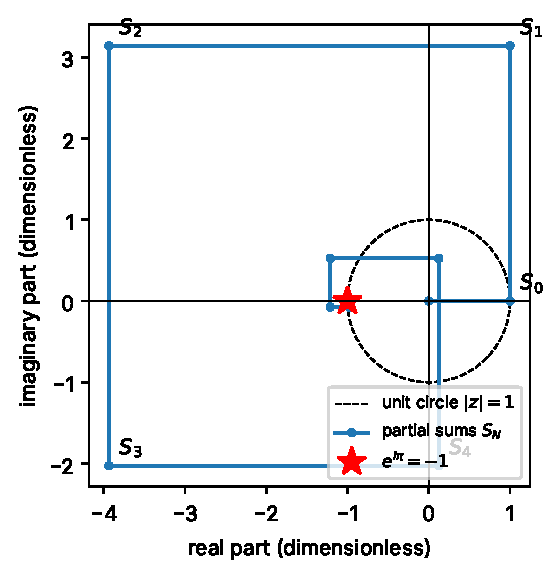
\includegraphics[width=0.85\linewidth]{figs/complex_euler_partial.pdf}
\caption{Partial sums $S_N=\sum_{n=0}^N(i\pi)^n/n!$ of the exponential series for $e^{i\pi}$, plotted in the complex plane for $N=0,\dots,14$. Consecutive steps are at right angles; the path spirals into $e^{i\pi}=-1$ (star). The dashed curve is the unit circle $\abs z=1$, on which every $e^{i\theta}$ with real $\theta$ lies.}
\label{fig:complex-euler-partial}
\end{figure}

\subsection{Consequences}

\emph{Special values.} From Eq.~\eqref{eq:complex-euler}:
\begin{equation}
e^{i\pi/2}=i,\qquad e^{i\pi}=-1,\qquad e^{2\pi i}=1,\qquad e^{i(\theta+2\pi)}=e^{i\theta}.\label{eq:complex-special}
\end{equation}
The second is the famous $e^{i\pi}+1=0$. The last says $e^{i\theta}$ is periodic in $\theta$ with period $2\pi$.

\emph{The unit circle.} For real $\theta$, $\abs{e^{i\theta}}=\sqrt{\cos^2\theta+\sin^2\theta}=1$. So $e^{i\theta}$ is always on the circle of radius 1, at angle $\theta$. Its conjugate is $\overline{e^{i\theta}}=\cos\theta-i\sin\theta=\cos(-\theta)+i\sin(-\theta)=e^{-i\theta}$.

\emph{Exponential polar form.} Equation~\eqref{eq:complex-polar} becomes
\begin{equation}
z=r\,e^{i\theta},\qquad r=\abs z,\ \theta=\arg z .\label{eq:complex-exppolar}
\end{equation}
The product rule Eq.~\eqref{eq:complex-prodpolar} now reads $r_1e^{i\theta_1}\,r_2e^{i\theta_2}=r_1r_2\,e^{i(\theta_1+\theta_2)}$: the old trigonometric addition formulas have become the law of exponents.

\emph{Exponentials of general complex numbers.} The exponent law holds for all complex numbers:
\begin{beyond}
For all complex $z$ and $w$, $e^{z}e^{w}=e^{z+w}$, where both sides are defined by the series \eqref{eq:complex-expdef}. The proof multiplies the two absolutely convergent series term by term (the ``Cauchy product'') and uses the binomial theorem; see~\cite{rhb}. For purely imaginary $z,w$ we proved it above, as Eq.~\eqref{eq:complex-Elaw}.
\end{beyond}
With $z=x$ real and $w=iy$ purely imaginary,
\begin{equation}
e^{x+iy}=e^{x}e^{iy}=e^{x}(\cos y+i\sin y).\label{eq:complex-exprect}
\end{equation}
So $\abs{e^{x+iy}}=e^{x}$ (using Eq.~\eqref{eq:complex-absprod} and $\abs{e^{iy}}=1$) and $\arg e^{x+iy}=y$. The real part of the exponent sets the size; the imaginary part sets the angle. Since $e^x>0$ for every real $x$, $e^{z}$ is never zero.

\emph{Derivative.} We found $\frac{\dd}{\dd\theta}e^{i\theta}=ie^{i\theta}$. More generally, for real $t$ and a complex constant $k=\alpha+i\omega$, Eq.~\eqref{eq:complex-exprect} gives $e^{kt}=e^{\alpha t}(\cos\omega t+i\sin\omega t)$, with real part $u(t)=e^{\alpha t}\cos\omega t$ and imaginary part $v(t)=e^{\alpha t}\sin\omega t$. By the real product rule,
\begin{align*}
u'(t)&=\alpha e^{\alpha t}\cos\omega t-\omega e^{\alpha t}\sin\omega t,\\
v'(t)&=\alpha e^{\alpha t}\sin\omega t+\omega e^{\alpha t}\cos\omega t .
\end{align*}
On the other hand, by Eq.~\eqref{eq:complex-mult},
\begin{align*}
k\,e^{kt}&=(\alpha+i\omega)\,e^{\alpha t}(\cos\omega t+i\sin\omega t)\\
&=e^{\alpha t}\bigl[(\alpha\cos\omega t-\omega\sin\omega t)+i(\alpha\sin\omega t+\omega\cos\omega t)\bigr],
\end{align*}
whose real part is $u'$ and whose imaginary part is $v'$. Hence $\frac{\dd}{\dd t}e^{kt}=u'+iv'=k\,e^{kt}$ (Problem~27 explores why this characterizes the exponential).

\begin{checkpoint}
What is $\abs{e^{i\theta}}$ for real $\theta$? What is $\abs{e^{2+3i}}$?
\end{checkpoint}
\checkanswer{$\abs{e^{i\theta}}=1$. By Eq.~\eqref{eq:complex-exprect}, $\abs{e^{2+3i}}=e^2\approx7.389$; the imaginary part $3$ only sets the angle.}

\begin{keyideas}
\item Taylor coefficients are $a_n=f^{(n)}(0)/n!$; this gives the series for $e^x$, $\cos x$, $\sin x$, Eqs.~\eqref{eq:complex-expseries}--\eqref{eq:complex-sinseries}.
\item The complex exponential is defined by the same series, Eq.~\eqref{eq:complex-expdef}.
\item Euler's formula $e^{i\theta}=\cos\theta+i\sin\theta$, Eq.~\eqref{eq:complex-euler}, follows by splitting the series into even and odd terms (allowed by absolute convergence, taken on trust).
\item $e^{x+iy}=e^x(\cos y+i\sin y)$: size $e^x$, angle $y$. Polar form is $z=re^{i\theta}$; $e^z$ is never zero.
\end{keyideas}

%==========================================================
\section{The exponential as rotation: phasors and oscillations}\label{sec:complex-rotation}
% DYK-BEGIN
\begin{didyouknow}{Phasors Power the Grid}
Charles Proteus Steinmetz, an engineer later at General Electric, showed in 1893 that alternating-current circuits become simple algebra if each sinusoidal voltage and current is represented by a complex number. Derivatives turn into multiplication by $i\omega$. His phasor method spread rapidly, and engineers still use it to analyze AC power networks, though they write $j$ instead of $i$.
\end{didyouknow}
% DYK-END

\subsection{Multiplying by $e^{i\alpha}$ rotates}

Take any $z=re^{i\theta}$ and a real angle $\alpha$. Then $e^{i\alpha}z=re^{i(\theta+\alpha)}$: same length, angle increased by $\alpha$. \emph{Multiplying by $e^{i\alpha}$ rotates the arrow counterclockwise by $\alpha$.} In components, with $z=x+iy$,
\begin{equation}
e^{i\alpha}(x+iy)=(\cos\alpha+i\sin\alpha)(x+iy)=(x\cos\alpha-y\sin\alpha)+i(x\sin\alpha+y\cos\alpha),\label{eq:complex-rotation}
\end{equation}
which you may recognize as the formula for rotating a 2D vector $(x,y)$ by angle $\alpha$. Multiplying by $i=e^{i\pi/2}$ rotates by $90^\circ$; that is why $iz$ in \Cref{fig:complex-plane} is perpendicular to $z$. Multiplying by $-1=e^{i\pi}$ rotates by $180^\circ$.

\subsection{Uniform circular motion and SHM}

Let $t$ be time, $R>0$ a radius and $\omega$ an angular frequency (radians per second). The complex number
\begin{equation}
z(t)=R\,e^{i\omega t}\label{eq:complex-circle}
\end{equation}
has constant modulus $R$ and argument $\omega t$ increasing at a steady rate, so it moves around a circle of radius $R$ counterclockwise, completing one turn when $\omega t=2\pi$, i.e. with period $2\pi/\omega$. Its real part is $x(t)=R\cos\omega t$, simple harmonic motion: SHM is the projection of uniform circular motion, now in one line of algebra. Differentiating, the velocity is $\dd z/\dd t=i\omega R e^{i\omega t}$: length $\omega R$ and direction rotated by $90^\circ$ from the position (tangent to the circle). The acceleration is $(i\omega)^2Re^{i\omega t}=-\omega^2z$: length $\omega^2R$, pointing toward the center. You recover the centripetal acceleration of first-year physics.

\subsection{Cosine and sine from exponentials}

Write Euler's formula for $\theta$ and for $-\theta$, using that cosine is even and sine is odd:
\[
e^{i\theta}=\cos\theta+i\sin\theta,\qquad e^{-i\theta}=\cos\theta-i\sin\theta .
\]
Adding the two lines and dividing by 2, or subtracting them and dividing by $2i$:
\begin{equation}
\cos\theta=\frac{e^{i\theta}+e^{-i\theta}}{2},\qquad\sin\theta=\frac{e^{i\theta}-e^{-i\theta}}{2i}.\label{eq:complex-cossin}
\end{equation}
Equivalently, $\cos\theta=\Re e^{i\theta}$ and $\sin\theta=\Im e^{i\theta}$. A real cosine is the sum of two arrows turning in opposite directions; their imaginary parts cancel and their real parts add. Formulas \eqref{eq:complex-cossin} turn every trigonometric identity into algebra with exponentials, as the samples below show.

\begin{figure}[htbp]\centering
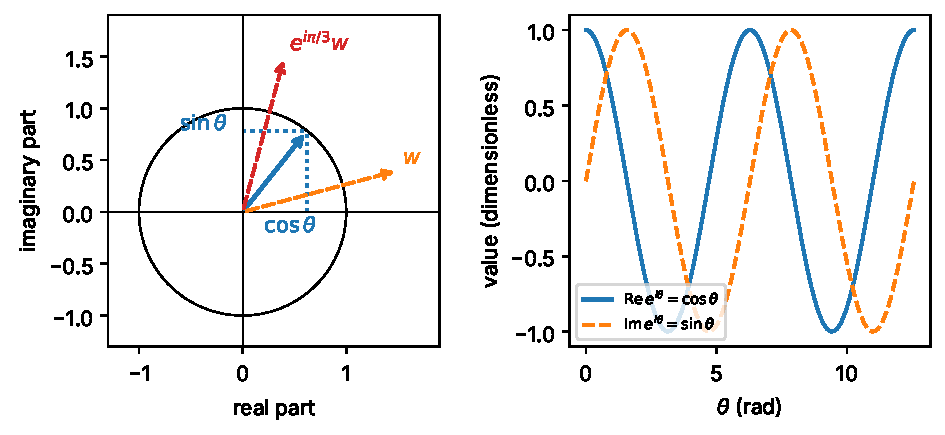
\includegraphics[width=0.85\linewidth]{figs/complex_rotation.pdf}
\caption{Left: the point $e^{i\theta}$ on the unit circle (here $\theta=0.9$ rad); its horizontal and vertical projections are $\cos\theta$ and $\sin\theta$. The dashed arrow $w=1.5+0.4i$ is rotated by $60^\circ$ when multiplied by $e^{i\pi/3}$. Right: as $\theta$ increases, the real and imaginary parts of $e^{i\theta}$ trace out $\cos\theta$ and $\sin\theta$ (angle $\theta$ in radians).}
\label{fig:complex-rotation}
\end{figure}

\subsection{Phasors}

A real sinusoid with amplitude $A>0$, angular frequency $\omega$ and phase constant $\phi$ can be written
\begin{equation}
A\cos(\omega t+\phi)=\Re\bigl[(Ae^{i\phi})\,e^{i\omega t}\bigr].\label{eq:complex-phasor}
\end{equation}
Check: $Ae^{i\phi}e^{i\omega t}=Ae^{i(\omega t+\phi)}$, whose real part is $A\cos(\omega t+\phi)$. The complex number $Ae^{i\phi}$ is the \textbf{complex amplitude} or \textbf{phasor}: its modulus is the amplitude and its argument is the phase. Because $\Re(u+v)=\Re u+\Re v$, adding sinusoids of the same frequency is the same as adding their phasors.

\begin{sample}{Adding two sinusoids of the same frequency}
Write $f(t)=3\cos\omega t+4\sin\omega t$ as a single cosine $A\cos(\omega t+\phi)$.

\textbf{Step 1:} Phasor of $3\cos\omega t$: by Eq.~\eqref{eq:complex-phasor} with $A=3,\phi=0$, it is $3$.

\textbf{Step 2:} Phasor of $4\sin\omega t$: since $\sin\omega t=\cos(\omega t-\pi/2)$, it is $4e^{-i\pi/2}=-4i$. (Check: $\Re(-4i\,e^{i\omega t})=\Re(-4i\cos\omega t+4\sin\omega t)=4\sin\omega t$.)

\textbf{Step 3:} Add the phasors: $3-4i$. Its modulus is $\sqrt{9+16}=5$; since its real part is positive, its principal argument is $\arctan(-4/3)\approx-0.927295$.

\textbf{Step 4:} So $f(t)=\Re[(3-4i)e^{i\omega t}]=5\cos(\omega t-0.927295)$.
\[
\boxed{3\cos\omega t+4\sin\omega t=5\cos(\omega t-0.927295)}
\]
\end{sample}

\begin{sample}{Two prime frequencies: beats}
Show that $\sin(t\log2)+\sin(t\log3)=2\sin\!\bigl(\tfrac{t\log6}{2}\bigr)\cos\!\bigl(\tfrac{t\log(3/2)}{2}\bigr)$, and find the period of the slow envelope.

\textbf{Step 1:} General identity. Let $A,B$ be real and set $P=(A+B)/2$, $Q=(A-B)/2$, so $A=P+Q$ and $B=P-Q$. Then
$e^{iA}+e^{iB}=e^{iP}(e^{iQ}+e^{-iQ})=2e^{iP}\cos Q$ and likewise $e^{-iA}+e^{-iB}=2e^{-iP}\cos Q$, using Eq.~\eqref{eq:complex-cossin}.

\textbf{Step 2:} By Eq.~\eqref{eq:complex-cossin},
\[
\sin A+\sin B=\frac{(e^{iA}+e^{iB})-(e^{-iA}+e^{-iB})}{2i}=\frac{2e^{iP}\cos Q-2e^{-iP}\cos Q}{2i}=2\cos Q\,\frac{e^{iP}-e^{-iP}}{2i}=2\sin P\cos Q .
\]

\textbf{Step 3:} Put $A=t\log2$, $B=t\log3$. Then $P=t(\log2+\log3)/2=t\log6/2$ and $Q=t(\log2-\log3)/2=-t\log(3/2)/2$. Cosine is even, so $\cos Q=\cos(t\log(3/2)/2)$.

\textbf{Step 4:} The fast factor oscillates with angular frequency $\log6/2\approx0.895880$; the envelope $2\cos(\cdot)$ has angular frequency $\log(3/2)/2\approx0.202733$. The loudness $\abs{2\cos Q}$ repeats when $Q$ changes by $\pi$, i.e. after $\Delta t=\pi/0.202733=2\pi/\log(3/2)\approx15.50$.

\[
\boxed{\sin(t\log2)+\sin(t\log3)=2\sin\!\bigl(\tfrac{t\log 6}{2}\bigr)\cos\!\bigl(\tfrac{t\log(3/2)}{2}\bigr),\quad\text{beat period}\approx15.50}
\]
Unlike beats between two frequencies in a whole-number ratio, this sum never repeats exactly. The ratio $\log 2/\log 3$ is irrational: if $\log2/\log3=b/a$ with positive integers $a,b$, then $a\log2=b\log3$, so $2^a=3^b$, which is impossible because $2^a$ is even and $3^b$ is odd. Sums of sinusoids with irrationally related frequencies are ``almost periodic''; Chapter~\ref{ch:fourier-series} shows that they never repeat. The paper's Eq.~(4) is such a sum.
\end{sample}

\begin{checkpoint}
Geometrically, what does multiplying a complex number by $i$ do? By $-i$?
\end{checkpoint}
\checkanswer{Multiplying by $i=e^{i\pi/2}$ rotates the arrow by $90^\circ$ counterclockwise; multiplying by $-i=e^{-i\pi/2}$ rotates it by $90^\circ$ clockwise. The length is unchanged in both cases.}

\begin{keyideas}
\item Multiplying by $e^{i\alpha}$ rotates by $\alpha$ without changing length; $Re^{i\omega t}$ is uniform circular motion with angular frequency $\omega$ and period $2\pi/\omega$.
\item $\cos\theta=(e^{i\theta}+e^{-i\theta})/2$ and $\sin\theta=(e^{i\theta}-e^{-i\theta})/(2i)$, Eq.~\eqref{eq:complex-cossin}.
\item A sinusoid $A\cos(\omega t+\phi)$ is the real part of the phasor $Ae^{i\phi}$ times $e^{i\omega t}$; same-frequency sinusoids add by adding phasors.
\item Trigonometric identities become exponent algebra.
\end{keyideas}

%==========================================================
\section{The complex logarithm and complex powers}\label{sec:complex-log}

\subsection{Undoing the exponential}

For a positive real number $x$, $\log x$ is the unique real $y$ with $e^y=x$. For a nonzero complex $z$, we look for complex $w=u+iv$ with $e^w=z$. Write $z=\abs z e^{i\theta}$ with $\theta=\operatorname{Arg}z$. By Eq.~\eqref{eq:complex-exprect}, $e^w=e^ue^{iv}$. For $e^ue^{iv}=\abs ze^{i\theta}$, the moduli must agree, $e^u=\abs z$, so $u=\log\abs z$ (an ordinary real logarithm, since $\abs z>0$). Then the unit-length factors must agree: $e^{iv}=e^{i\theta}$.

\textbf{Lemma.} For real $v,\theta$: $e^{iv}=e^{i\theta}$ if and only if $v=\theta+2\pi k$ for some integer $k$.
Proof: multiply both sides by $e^{-i\theta}$ (Eq.~\eqref{eq:complex-Elaw}): the condition becomes $e^{i(v-\theta)}=1$, that is $\cos(v-\theta)=1$ and $\sin(v-\theta)=0$ (Eq.~\eqref{eq:complex-equal}). The cosine equals 1 exactly at integer multiples of $2\pi$, where the sine is indeed 0.

So the solutions are
\begin{equation}
\log z=\log\abs z+i(\operatorname{Arg}z+2\pi k),\qquad k=0,\pm1,\pm2,\dots .\label{eq:complex-log}
\end{equation}
A nonzero complex number has infinitely many logarithms, differing by integer multiples of $2\pi i$. This is the logarithmic face of the fact that the argument is defined only up to $2\pi$. The choice $k=0$ gives the \textbf{principal logarithm},
\begin{equation}
\operatorname{Log}z=\log\abs z+i\operatorname{Arg}z,\qquad -\pi<\Im\operatorname{Log}z\le\pi .\label{eq:complex-Log}
\end{equation}
For positive real $z$ it is the ordinary logarithm (since $\operatorname{Arg}z=0$). And $\log 0$ is not defined at all, because $e^w$ is never zero.

\textbf{Branches, informally.} Picking one value of $k$ in a consistent way over a region of the plane is called choosing a \emph{branch} of the logarithm. The principal branch has a flaw: as $z$ crosses the negative real axis from above to below, $\operatorname{Arg}z$ jumps from nearly $\pi$ to nearly $-\pi$, so $\operatorname{Log}z$ jumps by $2\pi i$. The negative real axis is called the \emph{branch cut} of the principal logarithm. Away from it, $\operatorname{Log}$ changes continuously. When we follow a logarithm along a path that crosses the cut, we may instead switch $k$ to keep the logarithm continuous; Section~\ref{sec:complex-phase} does exactly that for arguments.

\begin{pitfall}
The rule $\log(zw)=\log z+\log w$ holds only up to a multiple of $2\pi i$. With principal values it can fail: $\operatorname{Log}(-1)=i\pi$, so $\operatorname{Log}(-1)+\operatorname{Log}(-1)=2\pi i$, but $\operatorname{Log}((-1)(-1))=\operatorname{Log}1=0$. The two sides differ by $2\pi i$.
\end{pitfall}

\subsection{Complex powers of positive numbers}

For a positive real number $a$ and any complex exponent $s$, we define
\begin{equation}
a^{s}=e^{s\log a},\label{eq:complex-power}
\end{equation}
where $\log a$ is the ordinary real logarithm. No ambiguity arises because $a$ is a positive real number with a single real logarithm. This definition agrees with the familiar one for real $s$ (since $e^{s\log a}=(e^{\log a})^s=a^s$ for real $s$), and by the exponent law it obeys $a^{s}a^{w}=e^{s\log a+w\log a}=a^{s+w}$. For two positive numbers $a,b$ it also obeys $(ab)^s=e^{s\log(ab)}=e^{s\log a+s\log b}=a^sb^s$.

For a complex base, say $i^i$, we would have to choose a logarithm of the base, and the answer depends on the branch. We will only ever need positive integer bases: the integers $k$ in $\sum k^{-s}$ and the primes $p$ in $p^{-s}$.

\begin{sample}{Logarithms and a surprising power}
Find $\operatorname{Log}(-2)$, $\operatorname{Log}(1+i)$, and the principal value of $i^i$ defined as $e^{i\operatorname{Log}i}$.

\textbf{Step 1:} $-2$ has modulus 2 and principal argument $\pi$, so $\operatorname{Log}(-2)=\log2+i\pi\approx0.693147+3.141593\,i$.

\textbf{Step 2:} $1+i$ has modulus $\sqrt2$ and argument $\pi/4$, so $\operatorname{Log}(1+i)=\log\sqrt2+i\pi/4=\tfrac12\log2+i\pi/4\approx0.346574+0.785398\,i$.

\textbf{Step 3:} $i$ has modulus 1 and argument $\pi/2$, so $\operatorname{Log}i=0+i\pi/2$. Then $i\operatorname{Log}i=i\cdot i\pi/2=-\pi/2$, a real number, and $i^i=e^{-\pi/2}\approx0.207880$.

\[
\boxed{\operatorname{Log}(-2)=\log2+i\pi,\quad\operatorname{Log}(1+i)=\tfrac12\log2+\tfrac{i\pi}{4},\quad i^i=e^{-\pi/2}\approx0.207880}
\]
With a different branch, $\log i=i(\pi/2+2\pi k)$ and $i^i=e^{-\pi/2-2\pi k}$: infinitely many real values. This is why we restrict complex powers to positive real bases.
\end{sample}

\begin{keyideas}
\item A nonzero $z$ has infinitely many logarithms $\log\abs z+i(\operatorname{Arg}z+2\pi k)$; the principal one has imaginary part in $(-\pi,\pi]$ and jumps by $2\pi i$ across the negative real axis.
\item $\log(zw)=\log z+\log w$ only up to multiples of $2\pi i$.
\item For positive real $a$ and complex $s$, $a^s=e^{s\log a}$ is unambiguous and obeys the usual exponent laws.
\end{keyideas}

%==========================================================
\section{Prime powers on the critical line}\label{sec:complex-primes}

\subsection{The arrow $p^{-s}$}

The zeta function and its relatives are built from quantities $k^{-s}$, with $k$ a positive integer and $s$ a complex variable. Following the universal convention of number theory, we write the real and imaginary parts of $s$ as
\[
s=\sigma+it,\qquad\sigma=\Re s,\quad t=\Im s .
\]
Here $\sigma$ is the Greek letter sigma. Note that $t$ is \emph{not} time in this context: it is a position along the vertical direction of the complex $s$-plane, the ``height''. All the nontrivial zeros used in this book have been verified numerically to lie on the line $\sigma=\tfrac12$, with heights $t=t_n$; whether every nontrivial zero does is the Riemann hypothesis, which is open (Chapter~\ref{ch:zeta}). (Zeta also has so-called trivial zeros on the negative real axis, Chapter~\ref{ch:zeta}; they play no role here.)

Apply the definition \eqref{eq:complex-power} with $a=k$ and exponent $-s$:
\begin{align}
k^{-s}&=e^{-s\log k}\nonumber\\
&=e^{-(\sigma+it)\log k}\nonumber\\
&=e^{-\sigma\log k}\,e^{-it\log k}\quad\text{(exponent law, Eq.~\eqref{eq:complex-exprect})}\nonumber\\
&=k^{-\sigma}\,e^{-it\log k}\quad\text{(since $e^{-\sigma\log k}=k^{-\sigma}$ for real $\sigma$)}.\label{eq:complex-pms}
\end{align}
This is the most important formula of the chapter for what follows. It splits $k^{-s}$ into a real, positive size $k^{-\sigma}$ and a unit-length rotating factor. So
\begin{equation}
\abs{k^{-s}}=k^{-\sigma},\qquad\arg k^{-s}=-t\log k\ (\text{mod }2\pi).\label{eq:complex-abspms}
\end{equation}
The size depends only on $\sigma$, the angle only on $t$. In real and imaginary parts,
\begin{equation}
k^{-s}=k^{-\sigma}\cos(t\log k)-i\,k^{-\sigma}\sin(t\log k).\label{eq:complex-pmsparts}
\end{equation}

\subsection{On the critical line}

On the vertical line $\sigma=\tfrac12$, which number theorists call the \textbf{critical line} (Chapter~\ref{ch:zeta} explains the name), Eq.~\eqref{eq:complex-abspms} gives for a prime $p$
\begin{equation}
\abs{p^{-s}}=p^{-1/2}=\frac1{\sqrt p}\qquad(\sigma=\tfrac12).\label{eq:complex-critmod}
\end{equation}
As $t$ increases, the arrow $p^{-s}$ keeps its length $1/\sqrt p$ and its angle $-t\log p$ decreases steadily: the arrow turns \emph{clockwise} around a circle of radius $1/\sqrt p$. Its angular rate, in radians per unit of $t$, is $\log p$. In the language of Section~\ref{sec:complex-rotation}, $p^{-s}$ rotates with \textbf{angular frequency $\log p$ in the variable $t$}, and its period in $t$ is
\begin{equation}
\text{period}=\frac{2\pi}{\log p}.\label{eq:complex-period}
\end{equation}
Larger primes give smaller circles and faster rotation (\Cref{tab:complex-primes} and \Cref{fig:complex-pminus-s}).

\begin{table}[htbp]\centering
\caption{The arrow $p^{-s}$ on the critical line $\sigma=\tfrac12$ for the first six primes: radius $1/\sqrt p$, angular frequency $\log p$ in $t$, and period $2\pi/\log p$.}\label{tab:complex-primes}
\begin{tabular}{cccc}
\toprule
$p$ & $1/\sqrt p$ & $\log p$ & $2\pi/\log p$\\
\midrule
2 & 0.7071 & 0.6931 & 9.0647\\
3 & 0.5774 & 1.0986 & 5.7192\\
5 & 0.4472 & 1.6094 & 3.9040\\
7 & 0.3780 & 1.9459 & 3.2289\\
11 & 0.3015 & 2.3979 & 2.6203\\
13 & 0.2774 & 2.5649 & 2.4496\\
\bottomrule
\end{tabular}
\end{table}

\begin{figure}[htbp]\centering
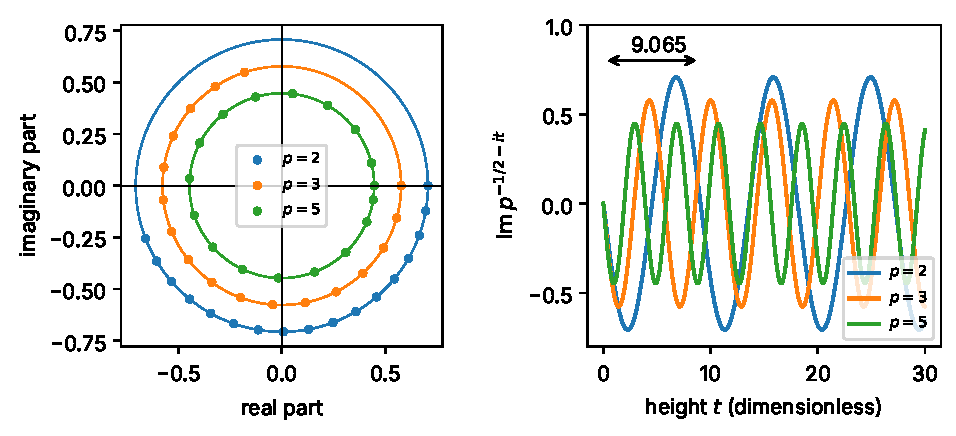
\includegraphics[width=0.85\linewidth]{figs/complex_pminus_s.pdf}
\caption{Left: as $t$ runs from 0 to 4 in steps of 0.25, the arrow $p^{-1/2-it}$ moves clockwise around a circle of radius $1/\sqrt p$, for $p=2,3,5$; dots mark the steps, and larger primes turn faster. Right: the imaginary parts $\Im p^{-1/2-it}=-p^{-1/2}\sin(t\log p)$ as functions of the height $t$ (dimensionless). The $p=2$ curve has period $2\pi/\log2\approx9.065$.}
\label{fig:complex-pminus-s}
\end{figure}

\subsection{Powers $p^{-ms}$ and harmonics}

Raise $p^{-s}$ to the $m$-th power ($m=1,2,3,\dots$). Applying the exponent law $e^{z}e^{w}=e^{z+w}$ $m-1$ times gives $(p^{-s})^m=(e^{-s\log p})^m=e^{-ms\log p}$, and since $m\log p=\log p^m$ this equals $e^{-s\log p^m}=(p^m)^{-s}$, which we write $p^{-ms}$. Then Eq.~\eqref{eq:complex-pms} with $k=p^m$, together with $(p^m)^{-\sigma}=p^{-m\sigma}$, gives
\begin{equation}
p^{-ms}=(p^m)^{-s}=p^{-m\sigma}\,e^{-imt\log p}.\label{eq:complex-pmms}
\end{equation}
On the critical line its length is $p^{-m/2}$ and its angular frequency in $t$ is $m\log p=\log p^m$: the $m$-th harmonic of the prime-$p$ rotation. Taking the imaginary part, with Eq.~\eqref{eq:complex-pmsparts},
\begin{equation}
\Im\bigl[p^{-ms}\bigr]=-p^{-m/2}\sin(mt\log p),\qquad\text{so}\qquad\frac{\sin(mt\log p)}{m\,p^{m/2}}=-\frac{1}{m}\Im\bigl[p^{-ms}\bigr]\quad(\sigma=\tfrac12).\label{eq:complex-oracleterm}
\end{equation}
The left-hand form is exactly the shape of each term in the paper's Eq.~(4). In particular our running example RE2, the prime-2 wave, is
\begin{equation}
-\frac1\pi\sum_{m=1}^{3}\frac{\sin(mt\log2)}{m\,2^{m/2}}=\frac1\pi\sum_{m=1}^3\frac1m\Im\bigl[2^{-m(1/2+it)}\bigr].\label{eq:complex-re2}
\end{equation}
Its three frequencies $\log2,\ 2\log2=\log4,\ 3\log2=\log8$ are whole-number multiples of $\log 2$, so RE2 repeats with the period of the slowest one, $2\pi/\log2\approx9.0647$ (Problem~18). Where the factor $-1/\pi$ and the sum over primes come from is the story of Chapters~\ref{ch:counting-zeros} and~\ref{ch:explicit-formula}.

\begin{sample}{The arrow $2^{-s}$ at the first zero}
Compute $2^{-\rho_1}$ for $\rho_1=\tfrac12+14.134725\,i$, giving its modulus, its principal argument and its real and imaginary parts.

\textbf{Step 1:} Modulus, Eq.~\eqref{eq:complex-critmod}: $\abs{2^{-\rho_1}}=2^{-1/2}\approx0.70711$.

\textbf{Step 2:} Argument, Eq.~\eqref{eq:complex-abspms}: $-t_1\log2=-14.134725\times0.693147\approx-9.79744$ rad.

\textbf{Step 3:} Reduce to $(-\pi,\pi]$ by adding $4\pi\approx12.56637$: $-9.79744+12.56637=2.76893$ rad.

\textbf{Step 4:} Real and imaginary parts: $\cos(2.76893)\approx-0.931360$ and $\sin(2.76893)\approx0.364101$, so $2^{-\rho_1}\approx0.70711(-0.931360+0.364101\,i)$.

\[
\boxed{2^{-\rho_1}\approx-0.65857+0.25746\,i,\qquad\abs{2^{-\rho_1}}\approx0.70711,\qquad\operatorname{Arg}2^{-\rho_1}\approx2.76893}
\]
\end{sample}

\begin{pycode}
import numpy as np
t1 = 14.134725141734695     # height of the first zeta zero
s = 0.5 + 1j * t1
for p in [2, 3, 5, 7, 11, 13]:
    w = p**(-s)              # Python computes exp(-s*log p)
    print(p, abs(w), np.angle(w), 2 * np.pi / np.log(p))
\end{pycode}

\begin{checkpoint}
On the critical line, what happens to $3^{-s}$ when $t$ increases by $2\pi/\log3\approx5.7192$? What happens to its modulus as $t$ changes?
\end{checkpoint}
\checkanswer{Its angle $-t\log3$ decreases by exactly $2\pi$, so $3^{-s}$ returns to the same value. Its modulus stays $1/\sqrt3\approx0.5774$ for every $t$.}

\begin{keyideas}
\item With $s=\sigma+it$, $k^{-s}=k^{-\sigma}e^{-it\log k}$: size $k^{-\sigma}$, angle $-t\log k$, Eqs.~\eqref{eq:complex-pms}--\eqref{eq:complex-abspms}.
\item On the critical line $\sigma=\tfrac12$, $p^{-s}$ is an arrow of length $1/\sqrt p$ turning clockwise with angular frequency $\log p$ in $t$, period $2\pi/\log p$.
\item $p^{-ms}$ has length $p^{-m/2}$ and frequency $m\log p=\log p^m$; $\sin(mt\log p)/(mp^{m/2})=-\Im[p^{-ms}]/m$, the building block of the paper's Eq.~(4).
\end{keyideas}

%==========================================================
\section{Functions of a complex variable and their zeros}\label{sec:complex-functions}

\subsection{What a complex function is}

A \textbf{function of a complex variable} assigns to each complex number $z$ (in some region) a complex number $f(z)$. Examples: $f(z)=z^2$, $f(z)=1/z$ (for $z\ne0$), $f(z)=e^z$, and $f(s)=1-2^{-s}$. The zeta function is another, defined in Chapter~\ref{ch:zeta}.

You cannot draw the graph of such a function in the usual way: input and output each need two real numbers, so the graph would live in four dimensions. Instead we use one of two tricks. (i) Split into two real functions of two real variables: writing $z=x+iy$, $f(z)=u(x,y)+iv(x,y)$ with $u=\Re f$ and $v=\Im f$. (ii) Plot the modulus $\abs{f}$ (a ``landscape'' over the plane) and, if needed, the argument.

For $f(z)=z^2$ with $z=x+iy$: $z^2=x^2+2ixy+i^2y^2=(x^2-y^2)+i(2xy)$, so $u=x^2-y^2$ and $v=2xy$.

\subsection{Zeros}

A \textbf{zero} of $f$ is a point $z_0$ with $f(z_0)=0$. By Eq.~\eqref{eq:complex-equal}, this means \emph{both} real equations
\begin{equation}
u(x_0,y_0)=0\qquad\text{and}\qquad v(x_0,y_0)=0\label{eq:complex-zero}
\end{equation}
hold at once. Equivalently, $\abs{f(z_0)}=0$, since $\abs f=\sqrt{u^2+v^2}$ vanishes only when $u$ and $v$ both vanish. Each equation alone typically holds along a curve in the plane; the zeros are where two such curves cross. Two equations in two unknowns usually have isolated solutions, so we expect the zeros of a complex function to be separate points that can be listed one by one, $\rho_1,\rho_2,\dots$, rather than lines or regions. This counting of equations is only a heuristic. The function $f(z)=\Re z$ assigns a complex number to each $z$, yet it vanishes on the whole imaginary axis: its imaginary part $v$ is $0$ everywhere, so one of the two equations imposes no condition at all.
\begin{beyond}
For \emph{analytic} functions, meaning those with a complex derivative $f'(z)=\lim_{h\to0}[f(z+h)-f(z)]/h$ as the complex number $h$ approaches $0$ from every direction in the plane, the zeros of a function that is not identically zero are isolated points. Polynomials, $e^z$, $1-2^{-s}$ and the zeta function (away from its pole at $s=1$, Chapter~\ref{ch:zeta}) are analytic; $\Re z$ is not. We take this theorem on trust; it is proved in the complex-variables chapters of~\cite{rhb}.
\end{beyond}

For $f(z)=z^2$: $v=2xy=0$ requires $x=0$ or $y=0$. If $y=0$, then $u=x^2=0$ forces $x=0$. If $x=0$, then $u=-y^2=0$ forces $y=0$. So the only zero is $z=0$: the curves $u=0$ (the diagonal lines $y=\pm x$) and $v=0$ (the two axes) cross only at the origin.

\subsection{Zeros of polynomials}

\textbf{The quadratic formula for complex numbers.} Take $az^2+bz+c=0$ with complex $a,b,c$ and $a\ne0$, and write $D=b^2-4ac$ for the discriminant. Completing the square uses only the commutative, associative and distributive laws, which hold for complex numbers (Section~\ref{sec:complex-arith}):
\begin{align*}
az^2+bz+c&=a\Bigl[z^2+\frac{b}{a}z+\frac{c}{a}\Bigr]\\
&=a\Bigl[\Bigl(z+\frac{b}{2a}\Bigr)^2-\frac{b^2}{4a^2}+\frac{c}{a}\Bigr]\quad\text{(since $(z+\tfrac{b}{2a})^2=z^2+\tfrac{b}{a}z+\tfrac{b^2}{4a^2}$)}\\
&=a\Bigl[\Bigl(z+\frac{b}{2a}\Bigr)^2-\frac{D}{4a^2}\Bigr]\quad\text{(since $-\tfrac{b^2}{4a^2}+\tfrac{4ac}{4a^2}=-\tfrac{D}{4a^2}$)}.
\end{align*}
Let $w$ be a complex number with $w^2=D$. (One always exists: if $D=re^{i\theta}$, take $w=\sqrt r\,e^{i\theta/2}$, whose square is $re^{i\theta}$ by Eq.~\eqref{eq:complex-prodpolar}.) Then $D/(4a^2)=(w/2a)^2$, and with $u=z+b/(2a)$ the bracket is $u^2-(w/2a)^2=(u-w/2a)(u+w/2a)$. Since $a\ne0$, the equation holds exactly when this product is zero. A product of complex numbers is zero only if a factor is zero: by Eq.~\eqref{eq:complex-absprod}, $\abs{u_1u_2}=\abs{u_1}\abs{u_2}$ vanishes only if $\abs{u_1}=0$ or $\abs{u_2}=0$. So $u=\pm w/(2a)$, that is
\[
z=\frac{-b\pm w}{2a},\qquad w^2=D .
\]
This is the familiar formula, with the square root of $D$ meaning either complex number whose square is $D$ (the $\pm$ covers the other one). For real coefficients and a negative discriminant $D<0$, the two square roots of $D$ are $\pm i\sqrt{\abs D}$ (check: $(i\sqrt{\abs D})^2=-\abs D=D$).

\textbf{Conjugate pairs.} If a polynomial $q(z)=c_0+c_1z+\dots+c_dz^d$ has \emph{real} coefficients and $q(z_0)=0$, then $q(\bar z_0)=0$ too. Proof: by Eq.~\eqref{eq:complex-conjrules}, conjugation passes through sums and products, and $\bar c_k=c_k$ for real $c_k$, so $\overline{q(z_0)}=\bar c_0+\bar c_1\bar z_0+\cdots+\bar c_d\bar z_0^{\,d}=q(\bar z_0)$. Since $q(z_0)=0$, $q(\bar z_0)=\bar0=0$. So the non-real roots of a real polynomial come in mirror-image pairs.

\begin{beyond}
The \emph{fundamental theorem of algebra}: every polynomial of degree $d\ge1$ with complex coefficients has exactly $d$ complex roots, counted with multiplicity. Complex numbers are therefore ``enough'' for polynomial equations: we never need to invent another kind of number. The proof uses methods beyond this book; see~\cite{rhb}. We will use the theorem in Chapter~\ref{ch:eigen}, where eigenvalues are roots of a polynomial.
\end{beyond}

\begin{sample}{A quadratic whose roots are the first zero and its mirror image}
Solve $z^2-z+\bigl(\tfrac14+t_1^2\bigr)=0$ with $t_1=14.134725$.

\textbf{Step 1:} Coefficients: $a=1$, $b=-1$, $c=\tfrac14+t_1^2\approx200.0405$.

\textbf{Step 2:} Discriminant: $D=b^2-4ac=1-4\bigl(\tfrac14+t_1^2\bigr)=1-1-4t_1^2=-4t_1^2<0$.

\textbf{Step 3:} The square roots of $D$ are $\pm i\sqrt{4t_1^2}=\pm 2it_1$.

\textbf{Step 4:} Quadratic formula: $z=\dfrac{1\pm2it_1}{2}=\tfrac12\pm it_1$.

\[
\boxed{z=\tfrac12+14.134725\,i\quad\text{and}\quad z=\tfrac12-14.134725\,i}
\]
The roots are $\rho_1$ and its conjugate $\bar\rho_1$, as the conjugate-pair theorem requires. The zeta zeros also come in conjugate pairs (Chapter~\ref{ch:zeta}); by convention we list only those with $t>0$.
\end{sample}

\subsection{The zeros of $1-2^{-s}$}

Our first example built from a prime is $f(s)=1-2^{-s}$. This factor reappears in Chapter~\ref{ch:zeta}. First a lemma.

\textbf{Lemma.} For complex $w$: $e^{w}=1$ if and only if $w=2\pi ik$ for some integer $k$.
Proof: write $w=u+iv$. Then $e^w=e^ue^{iv}$ has modulus $e^u$, which equals 1 only if $u=0$. Then $e^{iv}=1=e^{i0}$, which by the lemma of Section~\ref{sec:complex-log} means $v=2\pi k$.

\begin{sample}{Zeros built from the prime 2}
Find all zeros of $f(s)=1-2^{-s}$, first with the lemma and then by checking that real and imaginary parts both vanish.

\textbf{Step 1:} $f(s)=0$ means $2^{-s}=1$, i.e. $e^{-s\log2}=1$ (Eq.~\eqref{eq:complex-power}).

\textbf{Step 2:} By the lemma, $-s\log2=2\pi ik$, so $s=-2\pi ik/\log2$. As $k$ runs over all integers, so does $-k$; hence the zeros are $s=2\pi ik/\log 2$, $k=0,\pm1,\pm2,\dots$.

\textbf{Step 3:} Cross-check with real and imaginary parts. With $s=\sigma+it$, Eq.~\eqref{eq:complex-pmsparts} gives $f=\bigl[1-2^{-\sigma}\cos(t\log2)\bigr]+i\bigl[2^{-\sigma}\sin(t\log2)\bigr]$. The imaginary part vanishes only if $\sin(t\log2)=0$ (since $2^{-\sigma}>0$), i.e. $t\log2=\pi j$ for an integer $j$. Then $\cos(t\log2)=(-1)^j$, and the real part is $1-(-1)^j2^{-\sigma}$. For odd $j$ this is $1+2^{-\sigma}>0$, never zero. For even $j=2k$ it is $1-2^{-\sigma}$, zero only at $\sigma=0$. So $\sigma=0$ and $t=2\pi k/\log2$, as before.

\textbf{Step 4:} The zeros lie on the imaginary axis, equally spaced by $2\pi/\log 2\approx9.0647$: at $0,\pm9.0647i,\pm18.1294i,\dots$

\[
\boxed{1-2^{-s}=0\iff s=\frac{2\pi ik}{\log2},\ k\in\{0,\pm1,\pm2,\dots\}}
\]
The spacing is the period of the prime-2 rotation, \Cref{tab:complex-primes}. None of these zeros is on the critical line; on that line $\abs{2^{-s}}=1/\sqrt2<1$, so $2^{-s}$ can never equal 1.
\end{sample}

\begin{figure}[htbp]\centering
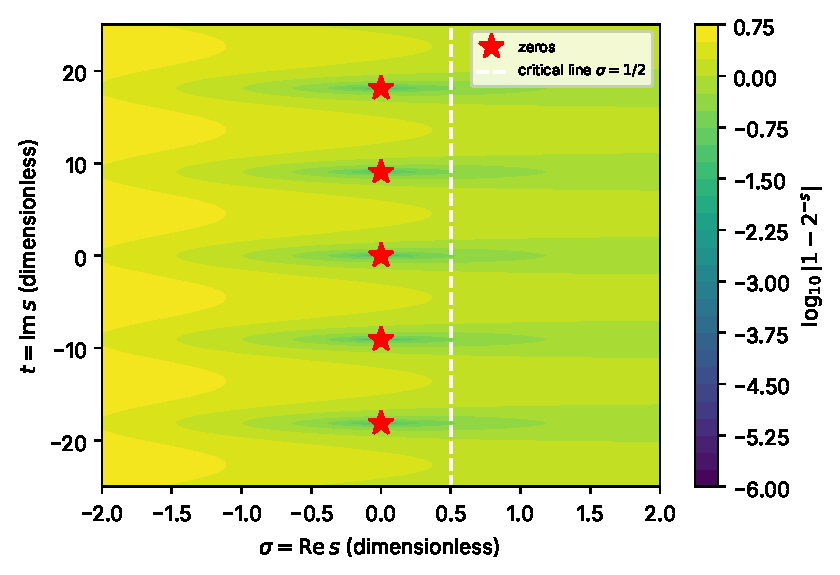
\includegraphics[width=0.85\linewidth]{figs/complex_zeros_1m2s.pdf}
\caption{The landscape of $\log_{10}\abs{1-2^{-s}}$ over the complex $s$-plane ($\sigma=\Re s$ horizontal, $t=\Im s$ vertical, both dimensionless). Dark wells are zeros: they sit on the imaginary axis at $t=2\pi k/\log2$, spaced by $9.065$ (stars). The dashed line is the critical line $\sigma=\tfrac12$, on which $\abs{1-2^{-s}}\ge1-1/\sqrt2$ and the function never vanishes.}
\label{fig:complex-zeros-1m2s}
\end{figure}

\begin{checkpoint}
Why does $e^z$ have no zeros anywhere in the complex plane?
\end{checkpoint}
\checkanswer{By Eq.~\eqref{eq:complex-exprect}, $\abs{e^{x+iy}}=e^x$, and $e^x>0$ for every real $x$. A number of positive modulus is not zero.}

\begin{keyideas}
\item A complex function $f(z)=u+iv$ can be studied through two real functions $u,v$ or through $\abs f$ and $\arg f$.
\item A zero requires $u=0$ and $v=0$ simultaneously (equivalently $\abs f=0$); zeros are typically isolated points.
\item Real polynomials have non-real roots in conjugate pairs; every polynomial of degree $d$ has $d$ complex roots (taken on trust).
\item $e^w=1$ iff $w=2\pi ik$; hence $1-2^{-s}$ vanishes exactly at $s=2\pi ik/\log2$.
\end{keyideas}

%==========================================================
\section{The argument of a function along a line}\label{sec:complex-phase}

\subsection{Arguments of products add}

Equation~\eqref{eq:complex-argprod} extends to any number of factors by applying it repeatedly: if $F=f_1f_2\cdots f_K$, then
\begin{equation}
\arg F=\arg f_1+\arg f_2+\cdots+\arg f_K\quad(\text{mod }2\pi),\label{eq:complex-argmany}
\end{equation}
and for a reciprocal, $\arg(1/f)=-\arg f$. A product of many factors has an angle that is a \emph{sum} of many angles. This simple fact is how the primes get into the counting of the zeta zeros: Chapter~\ref{ch:zeta} writes zeta as an infinite product with one factor per prime (the Euler product), each factor being $1/(1-p^{-s})$. Since $\arg(1/f)=-\arg f$, the argument of zeta becomes minus a sum over primes, $\arg\zeta(s)=-\sum_p\arg(1-p^{-s})$ (mod $2\pi$). This holds for $\Re s>1$, where the infinite product converges (Chapter~\ref{ch:zeta}). On the critical line the product does not converge, so the corresponding formula there is only formal (heuristic), as Chapter~\ref{ch:explicit-formula} discusses honestly.

\begin{sample}{Argument of a product, and of a prime factor}
(a) Find $\operatorname{Arg}\bigl[(1+i)(\sqrt3+i)\bigr]$ two ways. (b) Find $\operatorname{Arg}(1-2^{-s})$ on the critical line at the height $t^*$ where $t^*\log2=\pi/2$.

\textbf{Step 1:} (a) $\operatorname{Arg}(1+i)=\pi/4$ and $\operatorname{Arg}(\sqrt3+i)=\arctan(1/\sqrt3)=\pi/6$. Their sum $5\pi/12\approx1.308997$ lies in $(-\pi,\pi]$, so it is the principal argument of the product.

\textbf{Step 2:} Directly: $(1+i)(\sqrt3+i)=\sqrt3+i+i\sqrt3+i^2=(\sqrt3-1)+i(\sqrt3+1)\approx0.732051+2.732051\,i$. Then $\arctan(2.732051/0.732051)=\arctan(3.732051)$. To recognize this angle, divide the addition formulas for $\sin(A+B)$ and $\cos(A+B)$ and then divide top and bottom by $\cos A\cos B$: $\tan(A+B)=(\tan A+\tan B)/(1-\tan A\tan B)$. With $A=45^\circ$ ($\tan A=1$) and $B=30^\circ$ ($\tan B=1/\sqrt3$), $\tan75^\circ=\frac{1+1/\sqrt3}{1-1/\sqrt3}=\frac{\sqrt3+1}{\sqrt3-1}=\frac{(\sqrt3+1)^2}{3-1}=\frac{4+2\sqrt3}{2}=2+\sqrt3\approx3.732051$. Since $\arctan$ returns angles in $(-90^\circ,90^\circ)$, the argument is $75^\circ=5\pi/12$. Agreed.

\textbf{Step 3:} (b) $t^*=\pi/(2\log2)\approx2.266180$. On the critical line, $2^{-s}=2^{-1/2}e^{-it^*\log2}=2^{-1/2}e^{-i\pi/2}=-i/\sqrt2$.

\textbf{Step 4:} So $1-2^{-s}=1+i/\sqrt2$, with positive real part, and $\operatorname{Arg}(1-2^{-s})=\arctan(1/\sqrt2)\approx0.615480$.

\[
\boxed{\text{(a) }\tfrac{5\pi}{12}\approx1.308997;\qquad\text{(b) }\operatorname{Arg}(1-2^{-s})\big|_{t^*}=\arctan\tfrac1{\sqrt2}\approx0.615480}
\]
\end{sample}

\subsection{Following the argument continuously}

Suppose $f(t)$ is a complex number that depends continuously on a real parameter $t$ running over an interval (for instance, a function evaluated along the critical line, $f(\tfrac12+it)$) and is never zero along the way. A \textbf{continuous argument} of $f$ is a continuous real function $\alpha(t)$ with $f(t)=\abs{f(t)}e^{i\alpha(t)}$ for all $t$. Three facts:

\emph{It exists.} We take this on trust, with the following sketch.
\begin{beyond}
Two calculus theorems are used without proof (see~\cite{rhb}): a continuous function on a closed interval attains a minimum, and it is uniformly continuous there. Since $\abs{f(t)}$ is continuous and never zero on the closed interval $[t_a,t_b]$, it has a positive minimum $\mu$. By uniform continuity we can cut $[t_a,t_b]$ into finitely many pieces so short that on each piece $\abs{f(t)-f(t_j)}<\mu$, where $t_j$ is the left end of the piece. Then $\abs{f(t)/f(t_j)-1}<\mu/\abs{f(t_j)}\le1$, so $f(t)/f(t_j)$ lies in the disc of radius 1 about the point 1, which is inside the right half-plane. There $\operatorname{Arg}$ is continuous, so $\operatorname{Arg}f(t_j)+\operatorname{Arg}[f(t)/f(t_j)]$ is a continuous argument of $f$ on that piece (Eq.~\eqref{eq:complex-argprod}). At the end of each piece, the next piece's argument differs from it by a multiple of $2\pi$; subtracting that constant joins the pieces into one continuous argument.
\end{beyond}

\emph{It is unique up to a constant multiple of $2\pi$.} If $\alpha_1$ and $\alpha_2$ are both continuous arguments, their difference is continuous and, at every $t$, an integer multiple of $2\pi$ (by the lemma of Section~\ref{sec:complex-log}). Recall the intermediate value theorem of calculus: if $g$ is continuous on an interval $[t_a,t_b]$, then $g$ takes every value between $g(t_a)$ and $g(t_b)$. Let $g=\alpha_1-\alpha_2$, defined on the interval over which $t$ runs. If $g$ took two different values $2\pi j<2\pi j'$ at two points, it would also take every value between them, including $2\pi j+\pi$, which is not a multiple of $2\pi$. That is impossible, so $g$ is constant. Fixing $\alpha$ at one starting point fixes it everywhere.

\emph{For products it adds exactly.} If $\alpha$ and $\beta$ are continuous arguments of $f$ and $g$, then $fg=\abs f\abs g\,e^{i(\alpha+\beta)}$ and $\alpha+\beta$ is continuous, so $\alpha+\beta$ is a continuous argument of $fg$. With continuous arguments there is no ``mod $2\pi$'' left in Eq.~\eqref{eq:complex-argmany}.

The principal argument $\operatorname{Arg}$ is continuous as long as $f(t)$ avoids the negative real axis (Section~\ref{sec:complex-log}). When the path does cross that axis, $\operatorname{Arg}$ jumps by $2\pi$, and we must add or subtract $2\pi$ to remove the jump; numpy's \texttt{np.unwrap} does this. If the path circles around the origin, a continuous argument can grow without bound; counting such windings is the idea behind counting zeros in Chapter~\ref{ch:counting-zeros} (see also Problem~28).

\textbf{A continuous argument of $1-2^{-s}$ on the critical line.} Let $x=2^{-1/2-it}$, so $\abs x=1/\sqrt2$. Then $\Re(1-x)=1-\Re x\ge1-\abs x=1-1/\sqrt2>0$. So $1-2^{-s}$ stays in the right half-plane for all real $t$, never touches the negative real axis, and its principal argument is continuous and lies in $(-\pi/2,\pi/2)$. No unwrapping is needed.

\subsection{A preview: the phase of a prime factor is the prime-2 wave}

Here is a numerical observation that previews the central mechanism of Chapter~\ref{ch:explicit-formula}. Plot $-\frac1\pi\operatorname{Arg}(1-2^{-1/2-it})$ against $t$, and on the same axes plot RE2, the three-term prime-2 wave of Eq.~\eqref{eq:complex-re2}. \Cref{fig:complex-arg-prime2} shows that the two curves are nearly the same; a numerical computation (the code listing at the end of this subsection) finds that they differ by less than $0.05$ for all $t$ (they are both periodic with period $2\pi/\log 2$, so checking one period suffices). At $t^*$ of the last Sample Problem, for instance, the argument gives $-0.615480/\pi\approx-0.195913$ while RE2 gives $-\frac1\pi\bigl(\tfrac{1}{\sqrt2}-\tfrac{1}{3\cdot2^{3/2}}\bigr)\approx-0.187566$ (the $m=2$ term vanishes because $\sin\pi=0$).

\begin{figure}[htbp]\centering
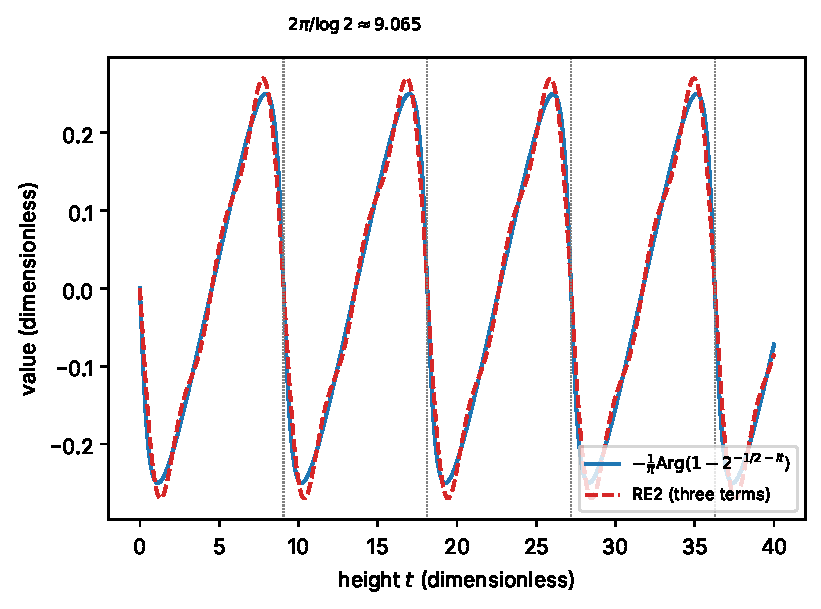
\includegraphics[width=0.85\linewidth]{figs/complex_arg_prime2.pdf}
\caption{Solid: minus the phase of the prime-2 factor, $-\frac1\pi\operatorname{Arg}(1-2^{-1/2-it})$, against the height $t$. Dashed: the three-term prime-2 wave RE2, $-\frac1\pi\sum_{m=1}^3\sin(mt\log2)/(m2^{m/2})$. They agree to within $0.05$; both repeat with period $2\pi/\log2\approx9.065$ (marked).}
\label{fig:complex-arg-prime2}
\end{figure}

The status of this observation: in this chapter it is a numerical observation. It becomes a theorem once we take one fact on trust.
\begin{beyond}
For a complex number $x$ with $\abs x<1$, the series $\mathcal S(x)=-(x+x^2/2+x^3/3+\cdots)$ converges, and $e^{\mathcal S(x)}=1-x$. For real $x$ in $(-1,1)$ this is the Taylor series $\log(1-x)=-(x+x^2/2+x^3/3+\cdots)$ derived in Chapter~\ref{ch:series}. The extension to complex $x$, including the identity $e^{\mathcal S(x)}=1-x$, is proved in the complex-variables chapters of~\cite{rhb}.
\end{beyond}
Given this, $\mathcal S(x)$ is one of the logarithms of $1-x$ in Eq.~\eqref{eq:complex-log}, and $\Im\mathcal S(x)$ is one of the arguments of $1-x$. Which one? Apply the triangle inequality, Eq.~\eqref{eq:complex-triangle}, repeatedly to a partial sum, using $\abs{x^m}=\abs x^m$ (Eq.~\eqref{eq:complex-absprod}):
\[
\Bigl\lvert x+\frac{x^2}{2}+\cdots+\frac{x^N}{N}\Bigr\rvert\le\abs x+\frac{\abs x^2}{2}+\cdots+\frac{\abs x^N}{N}.
\]
The right side is a partial sum of the real series for $-\log(1-\abs x)$; its terms are positive, so it never exceeds $-\log(1-\abs x)$. Letting $N\to\infty$, and using $\abs{\Im u}\le\abs u$ for any complex $u$, we get $\abs{\Im\mathcal S}\le\abs{\mathcal S}\le-\log(1-\abs x)$. For $\abs x=1/\sqrt2$ this is $-\log(1-1/\sqrt2)\approx1.228<\pi$. Arguments of the same number differ by multiples of $2\pi$, so only one of them lies in $(-\pi,\pi)$, and that one is the principal argument. Hence $\Im\mathcal S(x)=\operatorname{Arg}(1-x)$. With $x=2^{-1/2-it}$, Eq.~\eqref{eq:complex-oracleterm} gives $\Im x^m=-2^{-m/2}\sin(mt\log2)$, so $\operatorname{Arg}(1-2^{-s})=\sum_{m\ge1}\sin(mt\log2)/(m2^{m/2})$ exactly, and RE2 keeps the first three terms. Chapter~\ref{ch:explicit-formula} then does the same for every prime factor of zeta, which is where the paper's Eq.~(4) comes from (with an honest discussion of what is rigorous and what is not).

\begin{pycode}
import numpy as np, qmnt
t = qmnt.zeros(10)                 # RE1: heights of the first ten zeros
rho = 0.5 + 1j * t
print(np.abs(rho), np.angle(rho))  # moduli and principal arguments
tt = np.linspace(0, 40, 4001)
x = 2.0**(-0.5 - 1j * tt)
phase = -np.angle(1 - x) / np.pi
re2 = -sum(np.sin(m * tt * np.log(2)) / (m * 2**(m / 2))
           for m in (1, 2, 3)) / np.pi
print(np.max(np.abs(phase - re2)))  # below 0.05
\end{pycode}

\begin{keyideas}
\item The argument of a product is the sum of the arguments (mod $2\pi$), Eq.~\eqref{eq:complex-argmany}.
\item Along a path that avoids zeros, a continuous argument exists, is unique up to a constant $2\pi k$, and adds exactly over products.
\item On the critical line $1-2^{-s}$ stays in the right half-plane, so its principal argument is continuous; numerically, $-\frac1\pi\operatorname{Arg}(1-2^{-s})$ matches the prime-2 wave RE2 to within $0.05$ (proved later via the series for $\log(1-x)$).
\end{keyideas}

%==========================================================
\section{Paper connection}\label{sec:complex-paper}
% DYK-BEGIN
\begin{didyouknow}{Who Named $i$?}
The symbol $i$ for $\sqrt{-1}$ is due to Leonhard Euler, who used it in a memoir written in 1777 and published in 1794, after his death. Gauss later adopted it, which helped make it standard. Euler also introduced the letter $e$, popularized $\pi$, and found $e^{ix}=\cos x+i\sin x$. Every zeta zero in this book is written $\tfrac12+it_n$ in his notation.
\end{didyouknow}
% DYK-END

\paragraph{The zeros are complex numbers (Sec.~I, first sentence; Sec.~II~A).} The paper opens: ``The Hilbert--P\'olya conjecture proposes that the imaginary parts $t_n$ of the nontrivial zeros $\rho_n=\tfrac12+it_n$ of the Riemann zeta function are the spectrum of a self-adjoint operator''~\cite{soniR1}. You can now parse every symbol: $\rho_n$ is a complex number with real part $\tfrac12$ and imaginary part $t_n$, a real number. Sec.~II~A reports $t_1=14.134725141734695$ and $t_{1000}=1419.42248094599$; these are imaginary parts, as in our Sample Problem on $\abs{\rho_1}$. Writing every zero with real part $\tfrac12$ places them all on the vertical line $\sigma=\tfrac12$ of the complex plane (\Cref{fig:complex-critical}). That \emph{every} nontrivial zero lies on this line is the Riemann hypothesis, which is open (Chapter~\ref{ch:zeta}); the paper only uses zeros for which this has been verified numerically (a numerical observation, not a proof). From Sec.~II on, the paper works only with the real list $t_n$; the complex structure is hidden in that choice, and in the conjugate-pair symmetry that lets one keep only $t_n>0$.

\begin{figure}[htbp]\centering
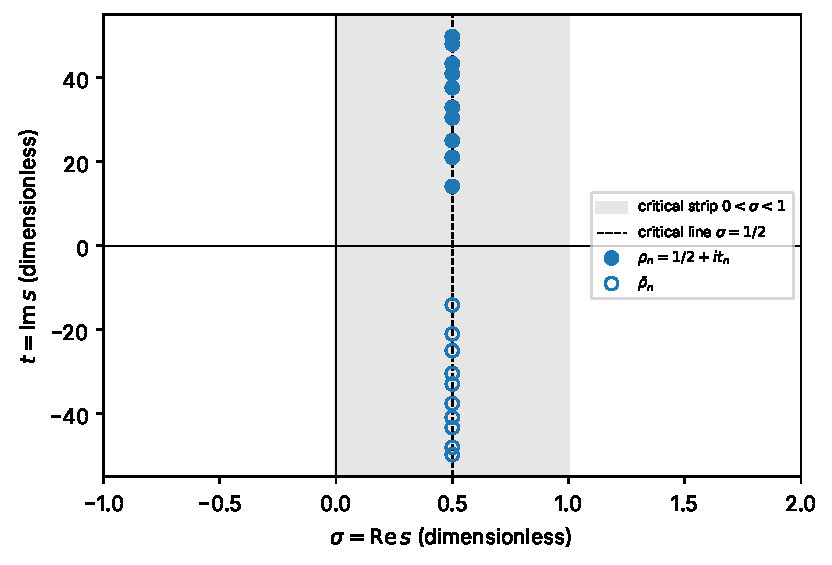
\includegraphics[width=0.85\linewidth]{figs/complex_critical_line.pdf}
\caption{The first ten nontrivial zeta zeros $\rho_n=\tfrac12+it_n$ (RE1, filled circles) and their conjugates $\bar\rho_n=\tfrac12-it_n$ (open circles) in the complex $s$-plane. The shaded band $0<\sigma<1$ is the critical strip and the dashed line is the critical line $\sigma=\tfrac12$ (Chapter~\ref{ch:zeta}). Note the very different scales of the two axes: the zeros are tall and thin in this picture, which is why $\operatorname{Arg}\rho_1$ is close to $90^\circ$.}
\label{fig:complex-critical}
\end{figure}

\paragraph{The sine terms of Eq.~(4).} The paper's arithmetic oracle, Eq.~(4) in Sec.~II~D, is
\[
N_{\rm fl}(t)=-\frac1\pi\sum_{p\in P}\sum_{m=1}^{3}\frac{\sin(mt\log p)}{m\,p^{m/2}}.
\]
By Eq.~\eqref{eq:complex-oracleterm}, every term is $-\Im[p^{-ms}]/m$ evaluated at $s=\tfrac12+it$. The factor $p^{-m/2}$ is the length of the arrow $p^{-ms}$ on the critical line, Eq.~\eqref{eq:complex-critmod}: it arises because the sum is evaluated at $s=\tfrac12+it$, that is at $\sigma=\tfrac12$, the real part shared by every zero $\rho_n$ that the paper uses, and there $\abs{p^{-ms}}=p^{-m\sigma}=1/\sqrt{p^m}$. The argument $mt\log p$ is the arrow's angle (up to sign), so $m\log p$ is an angular frequency in the variable $t$. So Eq.~(4) is a sum of rotating arrows, one family per prime, projected onto the imaginary axis. Chapters~\ref{ch:counting-zeros} and~\ref{ch:explicit-formula} derive why this sum approximates the fluctuating part of the zero count.

\paragraph{Frequencies $\log p^m$ (Secs.~II~D and IV; Table~IV; App.~A steps 20, 23).} The paper's abstract says that the sparse control C2 ``recovers frequencies at $\log p^m$''. Sec.~IV states this more carefully: every selected frequency ``lies within half the Fourier resolution of the training window of the logarithm of a prime power''. In our language $\log p^m=m\log p$ is the angular frequency of $p^{-ms}$ (Eq.~\eqref{eq:complex-pmms}). The smallest is $\log2\approx0.693$, period $9.0647$ in $t$; the controls search the range $0.05<\omega<8$ (Sec.~II~D). Note that $\omega=8$ corresponds to the prime power $q=e^8\approx2981$, which is consistent with the cutoff $q\le3000$ used in the alignment check of App.~A step 23. In the 800-zero C2 fit, the matched prime powers include $4=2^2$ and $8=2^3$, the $m=2,3$ harmonics of the prime 2 (Sec.~IV lists ``those up to 113 except 32, 64, and 81'').

\paragraph{The prime-2 wave and its period (Sec.~III continuation probe; Sec.~V).} The arithmetic-continuation probe of Sec.~III replaces the targets by ``a synthetic fluctuation consisting solely of the $p{=}2$ term of Eq.~(4)'': our RE2, Eq.~\eqref{eq:complex-re2}. It is a periodic signal with period $2\pi/\log 2\approx9.0647$ in $t$ (Problem~18). Sec.~V quotes this period: ``The dominant $p{=}2$ oscillation, period $2\pi/\log 2\approx9$ in $t$, is only $\sim$6--7 levels at these heights.'' Problem~30 checks that statement using the mean spacing derived in Chapter~\ref{ch:counting-zeros}: near height $t=650$, one period of the prime-2 wave spans about $6.7$ mean spacings. Our \Cref{fig:complex-arg-prime2} also shows that RE2 is, up to a tail smaller than $0.05$, minus $1/\pi$ times the phase of the single factor $1-2^{-s}$: the probe asks a fitted potential to continue the phase of one rotating arrow, and the paper finds that it cannot (held-out correlation $+0.07$, Sec.~III).

\paragraph{Complex eigenvalues (Sec.~II~E; Sec.~V; App.~A step 11).} The non-Hermitian classes of Sec.~II~E perturb $H\to H+iA$, an operator containing $i$ explicitly; the absorptive class models a term $-i\Gamma/2$. Such operators can have complex eigenvalues (the PT-odd class has a real spectrum to leading order, Sec.~II~E), and App.~A step 11 uses ``dense complex \texttt{eig}'' to compute them. The imaginary part of an eigenvalue $E-i\Gamma/2$ controls decay: in quantum mechanics a state with energy $E$ evolves with the factor $e^{-iEt}$ (Chapter~\ref{ch:schrodinger}, with $t$ now time), and by Eq.~\eqref{eq:complex-exprect} $\abs{e^{-i(E-i\Gamma/2)t}}=e^{-\Gamma t/2}$ (Problem~24). When Sec.~V reports that ``58\% of its widths have the wrong sign'', it refers to the sign of this imaginary part. Complex eigenvalues have no natural ``increasing order'' (Section~\ref{sec:complex-plane}), and in any case order does not tell which perturbed state came from which unperturbed one; the paper identifies states ``by overlap'' (Sec.~II~E (iii)), and Chapter~\ref{ch:non-hermitian} explains the procedure.

\paragraph{Phases and surrogates (Sec.~III; App.~A step 18).} The ``phase-randomized surrogate''~\cite{theiler} of Sec.~III is described as ``power spectrum kept exactly, no arithmetic content''. In Chapter~\ref{ch:fourier-transform} you will see that a sequence can be written as a sum of complex exponentials with complex coefficients; the surrogate keeps the modulus of each coefficient and replaces its argument by a random angle (``uniform phases'' in App.~A step 18). Modulus and argument, the two halves of polar form, are exactly the quantities being kept and scrambled.

\paragraph{Fig.~1.} The curves of Fig.~1 (fluctuations of zeros 370--460) are real numbers measured in mean spacings, but the six-prime prediction plotted there is built from six families of rotating arrows $p^{-ms}$ (presumably the first six primes, $p\le13$, \Cref{tab:complex-primes}; the paper says only ``six-prime''), projected onto the imaginary axis.

%==========================================================
\section{Summary}

\begin{itemize}
\item The imaginary unit satisfies $i^2=-1$ (Eq.~\eqref{eq:complex-i}); a complex number is $z=a+bi$ with real part $a$ and imaginary part $b$, both real. Multiplication: Eq.~\eqref{eq:complex-mult}.
\item In the complex plane $z$ is the point $(a,b)$. Conjugate $\bar z=a-bi$ (Eq.~\eqref{eq:complex-conj}), modulus $\abs z=\sqrt{a^2+b^2}$ (Eq.~\eqref{eq:complex-modulus}), $z\bar z=\abs z^2$ (Eq.~\eqref{eq:complex-zzbar2}), division by Eq.~\eqref{eq:complex-div}, $\abs{zw}=\abs z\abs w$ (Eq.~\eqref{eq:complex-absprod}), triangle inequality Eq.~\eqref{eq:complex-triangle}.
\item Polar form $z=r(\cos\theta+i\sin\theta)=re^{i\theta}$ (Eqs.~\eqref{eq:complex-polar}, \eqref{eq:complex-exppolar}); principal argument by Eq.~\eqref{eq:complex-atan2}; moduli multiply and arguments add (Eqs.~\eqref{eq:complex-prodpolar}, \eqref{eq:complex-argprod}); De Moivre Eq.~\eqref{eq:complex-demoivre}.
\item Taylor coefficients $a_n=f^{(n)}(0)/n!$ (Eq.~\eqref{eq:complex-taylorcoef}); complex exponential defined by the series Eq.~\eqref{eq:complex-expdef}; Euler's formula $e^{i\theta}=\cos\theta+i\sin\theta$ (Eq.~\eqref{eq:complex-euler}); $e^{x+iy}=e^x(\cos y+i\sin y)$ (Eq.~\eqref{eq:complex-exprect}).
\item Multiplication by $e^{i\alpha}$ is rotation (Eq.~\eqref{eq:complex-rotation}); $\cos\theta=(e^{i\theta}+e^{-i\theta})/2$, $\sin\theta=(e^{i\theta}-e^{-i\theta})/(2i)$ (Eq.~\eqref{eq:complex-cossin}); phasors (Eq.~\eqref{eq:complex-phasor}).
\item Logarithm $\log z=\log\abs z+i(\operatorname{Arg}z+2\pi k)$ (Eq.~\eqref{eq:complex-log}), principal branch Eq.~\eqref{eq:complex-Log}; powers of positive numbers $a^s=e^{s\log a}$ (Eq.~\eqref{eq:complex-power}).
\item With $s=\sigma+it$: $k^{-s}=k^{-\sigma}e^{-it\log k}$ (Eq.~\eqref{eq:complex-pms}), $\abs{k^{-s}}=k^{-\sigma}$ (Eq.~\eqref{eq:complex-abspms}); on the critical line $p^{-s}$ is an arrow of length $1/\sqrt p$ rotating with angular frequency $\log p$ in $t$, period $2\pi/\log p$ (Eqs.~\eqref{eq:complex-critmod}, \eqref{eq:complex-period}).
\item $\sin(mt\log p)/(mp^{m/2})=-\Im[p^{-ms}]/m$ on the critical line (Eq.~\eqref{eq:complex-oracleterm}); RE2 in this form is Eq.~\eqref{eq:complex-re2}.
\item Zeros of a complex function need both real and imaginary parts to vanish (Eq.~\eqref{eq:complex-zero}); real polynomials have conjugate-pair roots; $1-2^{-s}=0$ iff $s=2\pi ik/\log2$.
\item Arguments of products add (Eq.~\eqref{eq:complex-argmany}); continuous arguments along a path are unique up to $2\pi k$.
\end{itemize}

%==========================================================
\section{Problems}

\begin{problemlist}
\prob{1}{Let $z=2-3i$ and $w=-1+5i$. Compute $z+w$, $zw$ and $z/w$ in the form $a+bi$.}

\prob{1}{Simplify $i^7$, $i^{10}$, $i^{-1}$ and $i^{2027}$.}

\prob{1}{Find the modulus and principal argument of $-\sqrt3+i$, $-4$, $-2i$ and $3-3i$. Sketch each in the complex plane.}

\prob{1}{Write $2e^{i\pi/4}$, $5e^{-i\pi/2}$ and $e^{3\pi i}$ in the form $a+bi$. Then write $-1-i$ in the form $re^{i\theta}$ with $\theta$ the principal argument.}

\prob{1}{Starting from $z=a+bi$, show that $z+\bar z=2\Re z$, $z-\bar z=2i\Im z$ and $z\bar z=\abs z^2$. Use these to show that $z$ is real if and only if $z=\bar z$.}

\prob{1}{The second zeta zero is $\rho_2=\tfrac12+it_2$ with $t_2=21.022040$ (RE1). Compute $\abs{\rho_2}$ and $\operatorname{Arg}\rho_2$ (in radians and degrees). What is $\bar\rho_2$?}

\prob{1}{Evaluate $e^{i\pi}$, $e^{i\pi/2}$, $e^{2\pi i}$ and $e^{-i\pi/4}$ in the form $a+bi$.}

\prob{1}{For $z=5+12i$, find $\bar z$, $\abs z$, $1/z$ in the form $a+bi$, and $\abs{1/z}$.}

\prob{2}{Using components $z=a+bi$, $w=c+di$ (not polar form), prove that $\abs{zw}=\abs z\abs w$ and $\overline{zw}=\bar z\bar w$. Then, writing $u=e+fi$, prove the associative law $(zw)u=z(wu)$ by expanding both sides, and check it for $z=1+i$, $w=2-i$, $u=3i$ by computing both sides.}

\prob{2}{(a) Prove the reverse triangle inequality $\abs z-\abs w\le\abs{z-w}$. (Hint: apply Eq.~\eqref{eq:complex-triangle} to $z=(z-w)+w$.) (b) Use it to show that for $\sigma=\Re s>0$, $\abs{1-2^{-s}}\ge1-2^{-\sigma}>0$, so $1-2^{-s}$ has no zeros in the right half-plane. Compare with \Cref{fig:complex-zeros-1m2s}.}

\prob{2}{Expand $(\cos\theta+i\sin\theta)^3$ with the binomial theorem and compare with De Moivre's formula to derive $\cos3\theta=4\cos^3\theta-3\cos\theta$ and $\sin3\theta=3\sin\theta-4\sin^3\theta$.}

\prob{2}{Using Eq.~\eqref{eq:complex-cossin}, prove $\cos a\cos b=\tfrac12[\cos(a-b)+\cos(a+b)]$ and $\sin a\sin b=\tfrac12[\cos(a-b)-\cos(a+b)]$.}

\prob{2}{Use Eq.~\eqref{eq:complex-cossin} to write $\cos^2(\omega t)$ as a constant plus a cosine, and hence show that its average over one period $2\pi/\omega$ is $\tfrac12$. (This is why the rms of a sinusoid of amplitude $A$ is $A/\sqrt2$.)}

\prob{2}{(a) Find all three solutions of $z^3=1$ by writing $z=re^{i\theta}$ and $1=e^{2\pi ik}$. (b) Find all four solutions of $z^4=-16$. Sketch both sets; what shape do they form?}

\prob{2}{Find the principal values of $\operatorname{Log}(-e)$, $\operatorname{Log}(2i)$, $i^i=e^{i\operatorname{Log}i}$ and $2^i=e^{i\log2}$. Give numerical values to five decimals.}

\prob{2}{(Paper.) The six-prime oracle of the paper's Fig.~1 and Table~V uses six primes; the natural reading is the first six, $2,3,5,7,11,13$. For each, compute the radius of the circle traced by $p^{-s}$ on the critical line and its period in $t$. Which prime's arrow has the largest amplitude? Which turns fastest? Compare your table with \Cref{tab:complex-primes}.}

\prob{2}{(Paper.) Show that on the critical line $\sin(mt\log p)/(m\,p^{m/2})=-\Im[p^{-ms}]/m$. Hence rewrite the paper's Eq.~(4) as $N_{\rm fl}(t)=\frac1\pi\sum_{p\in P}\sum_{m=1}^3\frac1m\Im\bigl[p^{-m(1/2+it)}\bigr]$.}

\prob{2}{(Paper.) For the prime-2 wave RE2, list the angular frequencies of its three terms, write each as $\log q$ for an integer $q$, and give each term's period in $t$. Explain why the sum is periodic and find its period. (The paper's abstract says that the sparse control C2 recovers frequencies at $\log p^m$; Sec.~IV says that each selected frequency lies within half the Fourier resolution of the training window of the logarithm of a prime power.)}

\prob{2}{Find all zeros of (a) $f(s)=1-3^{-s}$ and (b) $g(s)=1+2^{-s}$. Where do they lie, and how far apart are neighboring zeros?}

\prob{2}{For $f(z)=z^2-1$ with $z=x+iy$, find $u=\Re f$ and $v=\Im f$. Sketch the curves $u=0$ and $v=0$ and locate their intersections. Check that these are the zeros you expect.}

\prob{2}{Prove that if a polynomial with real coefficients has a root $z_0$, then $\bar z_0$ is also a root. Apply this to $z^2-z+(\tfrac14+t_n^2)$ for any real $t_n$.}

\prob{2}{(Computational.) Using qmnt or numpy, form $\rho_n=\tfrac12+it_n$ for the ten zeros of RE1 (\texttt{qmnt.zeros(10)}) and compute $2^{-\rho_n}$ for each. Print the modulus and the principal argument. Explain why every modulus is the same, and give the argument for $n=1$ and $n=2$.}

\prob{2}{(Computational.) Using numpy, plot $-\frac1\pi\operatorname{Arg}(1-2^{-1/2-it})$ and RE2 on $0\le t\le40$ and compute the largest difference between them. Show that each omitted term $\frac1\pi\sin(mt\log2)/(m2^{m/2})$ with $m\ge4$ has size at most $1/(\pi m2^{m/2})$, sum these bounds numerically for $m=4,\dots,200$, and compare with your observed maximum.}

\prob{2}{(Paper.) In quantum mechanics a state of complex energy $\mathcal E=E-i\Gamma/2$ ($E,\Gamma$ real) carries the time factor $e^{-i\mathcal Et}$, $t$ being time. Show that $\abs{e^{-i\mathcal Et}}=e^{-\Gamma t/2}$ and that the probability $\abs{e^{-i\mathcal Et}}^2$ decays as $e^{-\Gamma t}$. For $E=100$ and $\Gamma=1$ (units with $\hbar=1$), when has the modulus fallen to one half? The probability? Why does Sec.~V of the paper call $\Gamma<0$ the ``wrong sign''?}

\prob{2}{(Paper, computational.) Show that for any zero on the critical line, $1-\rho_n=\bar\rho_n$, and hence $\rho_n(1-\rho_n)=\tfrac14+t_n^2$ is real and positive. Using \texttt{qmnt.zeros(10)}, verify numerically that $\rho_n(1-\rho_n)-(\tfrac14+t_n^2)$ vanishes to rounding error for $n=1,\dots,10$, and report the value of $\rho_1(1-\rho_1)$. (The symmetry $s\leftrightarrow1-s$ appears in the functional equation of Chapter~\ref{ch:zeta}.)}

\prob{2}{A particle moves on a circle of radius $R=0.5$ m at angular frequency $\omega=4$ rad/s, with position $z(t)=Re^{i\omega t}$ in the complex plane (meters). Find its velocity and acceleration as complex numbers, and their magnitudes. Show that the acceleration points toward the center.}

\prob{3}{Let $E(\theta)=\cos\theta+i\sin\theta$. (a) Show that $\overline{E(\theta)}$ satisfies $\frac{\dd}{\dd\theta}\overline{E}=-i\overline E$. (b) Suppose $F(\theta)$ is any differentiable complex function with $F'=iF$ and $F(0)=1$. By differentiating $F\overline E$, show that $F\overline E=1$, and deduce $F=E$. This gives a second proof that the only ``exponential with rate $i$'' is $\cos\theta+i\sin\theta$.}

\prob{3}{Use the finite geometric sum to show $\sum_{k=0}^{n-1}e^{ik\theta}=\dfrac{e^{in\theta}-1}{e^{i\theta}-1}$ for $e^{i\theta}\ne1$. By factoring $e^{in\theta/2}$ from the numerator and $e^{i\theta/2}$ from the denominator, derive $\sum_{k=0}^{n-1}\cos k\theta=\dfrac{\sin(n\theta/2)\cos((n-1)\theta/2)}{\sin(\theta/2)}$. Check numerically for $n=5$, $\theta=0.7$. (This sum reappears in Chapter~\ref{ch:fourier-transform}.)}

\prob{3}{Let $f(t)=1-re^{-it}$ with $r>0$ fixed and $t$ running from 0 to $2\pi$. (a) Show that $f(t)$ traces a circle of radius $r$ centered at 1, clockwise. (b) For $r<1$, show that the continuous argument of $f$ returns to its starting value at $t=2\pi$. (c) For $r>1$, show that it changes by $-2\pi$. (d) Using numpy's \texttt{np.unwrap}, confirm (b) and (c) numerically for $r=1/\sqrt2$ and $r=2$. Relate (b) to the absence of branch jumps in $\operatorname{Arg}(1-2^{-1/2-it})$.}



\prob{3}{(Paper.) Take as given (it is derived in Chapter~\ref{ch:counting-zeros}) that the local mean spacing of the zeros at height $t$ is $2\pi/\log(t/2\pi)$. How many mean spacings does one period $2\pi/\log2$ of the prime-2 wave span at $t=300$ and at $t=650$? Compare with the paper's statement in Sec.~V that the $p=2$ oscillation is ``only $\sim$6--7 levels at these heights'', and explain in words why the number of levels per period grows with height.}

\end{problemlist}

%==========================================================
\section{Answers to selected problems}

\textbf{1.} $z+w=1+2i$. $zw=-2+10i+3i-15i^2=13+13i$. $z/w=\dfrac{(2-3i)(-1-5i)}{1+25}=\dfrac{-2-10i+3i+15i^2}{26}=\dfrac{-17-7i}{26}\approx-0.653846-0.269231\,i$.

\textbf{2.} $7=4+3$, so $i^7=i^3=-i$. $10=8+2$, so $i^{10}=-1$. $i^{-1}=-i$ (since $i(-i)=1$). $2027=4\cdot506+3$, so $i^{2027}=-i$.

\textbf{3.} $-\sqrt3+i$: modulus 2, $a<0,b>0$, so $\operatorname{Arg}=\arctan(-1/\sqrt3)+\pi=-\pi/6+\pi=5\pi/6$. $-4$: modulus 4, argument $\pi$. $-2i$: modulus 2, argument $-\pi/2$. $3-3i$: modulus $3\sqrt2\approx4.2426$, argument $-\pi/4$.

\textbf{4.} $2e^{i\pi/4}=2(\tfrac{\sqrt2}2+i\tfrac{\sqrt2}2)=\sqrt2+i\sqrt2$. $5e^{-i\pi/2}=-5i$. $e^{3\pi i}=\cos3\pi+i\sin3\pi=-1$. $-1-i=\sqrt2e^{-3i\pi/4}$.

\textbf{5.} Eqs.~\eqref{eq:complex-zpluszbar}--\eqref{eq:complex-zzbar} written out. If $z=\bar z$, then $z-\bar z=2i\Im z=0$, so $\Im z=0$ and $z$ is real; conversely a real $z$ has $\bar z=z$.

\textbf{6.} $\abs{\rho_2}^2=0.25+21.022040^2=0.25+441.926166=442.176166$, so $\abs{\rho_2}\approx21.0280$. $\operatorname{Arg}\rho_2=\pi/2-\arctan(0.5/21.022040)\approx1.570796-0.023780=1.547016$ rad $\approx88.64^\circ$. $\bar\rho_2=\tfrac12-21.022040\,i$.

\textbf{7.} $e^{i\pi}=-1$; $e^{i\pi/2}=i$; $e^{2\pi i}=1$; $e^{-i\pi/4}=\tfrac{\sqrt2}2-i\tfrac{\sqrt2}2\approx0.70711-0.70711\,i$.

\textbf{8.} $\bar z=5-12i$. $\abs z=\sqrt{25+144}=\sqrt{169}=13$. By Eq.~\eqref{eq:complex-div}, $1/z=\bar z/\abs z^2=(5-12i)/169\approx0.029586-0.071006\,i$. By Eq.~\eqref{eq:complex-absprod}, $\abs{1/z}=1/\abs z=1/13\approx0.076923$.

\textbf{9.} $zw=(ac-bd)+(ad+bc)i$, so $\abs{zw}^2=(ac-bd)^2+(ad+bc)^2=a^2c^2-2abcd+b^2d^2+a^2d^2+2abcd+b^2c^2=(a^2+b^2)(c^2+d^2)$; take square roots. For the conjugate, see the computation before Eq.~\eqref{eq:complex-conjrules}. Associativity in general, with $u=e+fi$: $(zw)u$ has real part $(ac-bd)e-(ad+bc)f=ace-bde-adf-bcf$ and imaginary part $(ac-bd)f+(ad+bc)e=acf-bdf+ade+bce$. Next, $wu=(ce-df)+(cf+de)i$, so $z(wu)$ has real part $a(ce-df)-b(cf+de)=ace-adf-bcf-bde$ and imaginary part $a(cf+de)+b(ce-df)=acf+ade+bce-bdf$. The same four products appear in each part, so the two sides are equal. Numerical case: $zw=(1+i)(2-i)=2-i+2i-i^2=3+i$, $(zw)u=(3+i)3i=9i+3i^2=-3+9i$; $wu=(2-i)3i=6i+3=3+6i$, $z(wu)=(1+i)(3+6i)=3+6i+3i+6i^2=-3+9i$. Equal.

\textbf{11.} Binomial expansion: $(\cos\theta+i\sin\theta)^3=\cos^3\theta+3i\cos^2\theta\sin\theta+3i^2\cos\theta\sin^2\theta+i^3\sin^3\theta=(\cos^3\theta-3\cos\theta\sin^2\theta)+i(3\cos^2\theta\sin\theta-\sin^3\theta)$. By De Moivre this equals $\cos3\theta+i\sin3\theta$; equate parts (Eq.~\eqref{eq:complex-equal}). Then use $\sin^2\theta=1-\cos^2\theta$: real part $\cos^3\theta-3\cos\theta(1-\cos^2\theta)=4\cos^3\theta-3\cos\theta$; with $\cos^2\theta=1-\sin^2\theta$: imaginary part $3(1-\sin^2\theta)\sin\theta-\sin^3\theta=3\sin\theta-4\sin^3\theta$.

\textbf{13.} $\cos^2(\omega t)=\bigl(\tfrac{e^{i\omega t}+e^{-i\omega t}}2\bigr)^2=\tfrac{e^{2i\omega t}+2+e^{-2i\omega t}}4=\tfrac12+\tfrac12\cos(2\omega t)$. Over one period $2\pi/\omega$, $\cos(2\omega t)$ completes two full cycles and averages to zero, so the average is $\tfrac12$. The rms of $A\cos\omega t$ is $\sqrt{A^2/2}=A/\sqrt2$.

\textbf{15.} $\operatorname{Log}(-e)=\log e+i\pi=1+i\pi\approx1+3.14159\,i$. $\operatorname{Log}(2i)=\log2+i\pi/2\approx0.69315+1.57080\,i$. $i^i=e^{-\pi/2}\approx0.20788$. $2^i=\cos(\log2)+i\sin(\log2)\approx0.76924+0.63896\,i$.

\textbf{17.} By Eq.~\eqref{eq:complex-pmms} with $\sigma=\tfrac12$, $p^{-ms}=p^{-m/2}[\cos(mt\log p)-i\sin(mt\log p)]$, so $\Im[p^{-ms}]=-p^{-m/2}\sin(mt\log p)$; divide by $-m$. Substituting into Eq.~(4): $-\frac1\pi\sum\frac{\sin(mt\log p)}{mp^{m/2}}=-\frac1\pi\sum\bigl(-\frac1m\Im[p^{-ms}]\bigr)=\frac1\pi\sum\frac1m\Im[p^{-ms}]$.

\textbf{19.} (a) $3^{-s}=1\iff-s\log3=2\pi ik$, so $s=2\pi ik/\log3$: on the imaginary axis, spacing $2\pi/\log3\approx5.7192$. (b) $2^{-s}=-1=e^{i\pi(2k+1)}$ (using the lemma of Section~\ref{sec:complex-log}: $e^{w}=-1$ iff $w=i\pi+2\pi ik$, from $e^{w-i\pi}=1$), so $-s\log2=i\pi(2k+1)$ and $s=-i\pi(2k+1)/\log2$: on the imaginary axis at odd multiples of $\pi/\log2\approx4.5324$, spacing $9.0647$, interleaved halfway between the zeros of $1-2^{-s}$.

\textbf{21.} See the conjugate-pair proof in Section~\ref{sec:complex-functions}. The polynomial $z^2-z+(\tfrac14+t_n^2)$ has real coefficients and root $\tfrac12+it_n$ (as in the Sample Problem), so $\tfrac12-it_n$ is also a root.

\textbf{23.} Each term has $\abs{\sin}\le1$, so its size is at most $1/(\pi m2^{m/2})$. The sum of these bounds for $m\ge4$ is about $0.0487$, so the two curves can never differ by more than $0.0487$; the observed maximum on a fine grid is below this bound. (Exact identity behind the figure: the argument after \Cref{fig:complex-arg-prime2}, which uses the fact stated in the \texttt{beyond} box there.)

\textbf{25.} On the critical line $\rho_n=\tfrac12+it_n$, so $1-\rho_n=\tfrac12-it_n=\bar\rho_n$. Hence $\rho_n(1-\rho_n)=\rho_n\bar\rho_n=\abs{\rho_n}^2=\tfrac14+t_n^2$ by Eq.~\eqref{eq:complex-zzbar2}, which is real and positive. Numerically the difference $\rho_n(1-\rho_n)-(\tfrac14+t_n^2)$ is at the level of rounding error for all ten zeros, and $\rho_1(1-\rho_1)\approx200.040451$ (compare $\abs{\rho_1}^2$ in the Sample Problem on $\rho_1$).

\textbf{26.} $v=\dd z/\dd t=i\omega Re^{i\omega t}$, magnitude $\omega R=2$ m/s, direction $90^\circ$ ahead of the position (tangent). $a=\dd v/\dd t=(i\omega)^2Re^{i\omega t}=-\omega^2z$, magnitude $\omega^2R=8$ m/s$^2$; the factor $-1$ means it points from $z$ back toward the origin, the center of the circle.

\textbf{27.} (a) $\overline E=\cos\theta-i\sin\theta$, derivative $-\sin\theta-i\cos\theta=-i(\cos\theta-i\sin\theta)=-i\overline E$. (b) $(F\overline E)'=F'\overline E+F\overline E'=iF\overline E-iF\overline E=0$, so $F\overline E$ is constant, equal to its value $F(0)\overline{E(0)}=1$ at $\theta=0$. Since $E\overline E=\abs E^2=1$, multiply $F\overline E=1$ by $E$: $F=E$.

\textbf{29.} (a) $\abs{f(t)-1}=\abs{-re^{-it}}=r$, so $f$ is on the circle of radius $r$ about 1; the angle of $-re^{-it}=re^{i(\pi-t)}$ is $\pi-t$, decreasing, so the motion is clockwise. (b) For $r<1$ the circle lies in the half-plane $\Re f\ge1-r>0$; the principal argument is continuous there and is a continuous argument, so it returns to $\operatorname{Arg}f(0)$ at $t=2\pi$. (c) For $r>1$ the circle encloses the origin. As $f(t)$ goes once clockwise around it, the arrow from the origin to $f(t)$ makes one full clockwise turn, so the continuous argument changes by $-2\pi$. (d) \texttt{np.unwrap(np.angle(f))} ends where it started for $r=1/\sqrt2$, and $2\pi$ lower for $r=2$. With $r=1/\sqrt2$ and $t\log2$ in place of $t$, this is $1-2^{-1/2-it}$, which is why its argument needs no unwrapping.

\textbf{30.} At $t=300$: $\log(300/2\pi)\approx3.8659$, mean spacing $\approx1.6253$, and $9.0647/1.6253\approx5.58$ spacings per period. At $t=650$: $\log(650/2\pi)\approx4.6391$, spacing $\approx1.3544$, giving $\approx6.69$. The paper's ``$\sim$6--7 levels'' matches the upper part of the fitted range: the 400th zero sits at $t_{400}\approx680$ (from \texttt{qmnt.zeros(400)}), where one period spans $(2\pi/\log2)/(2\pi/\log(t_{400}/2\pi))=\log(t_{400}/2\pi)/\log2\approx6.8$ spacings. The period in $t$ is fixed, while the zeros crowd together as $t$ grows (the spacing shrinks like $1/\log t$), so more levels fit into one period.




